\documentclass[a4paper]{ctexart}
\usepackage{xeCJK}
\usepackage{setspace}
\usepackage{graphicx,wrapfig}
\usepackage{fontspec,xunicode,xltxtra}
\usepackage{fancyhdr,titlesec,titletoc}
\usepackage[titletoc]{appendix}
\usepackage[top=29mm,bottom=29mm,left=31.8mm,right=31.8mm]{geometry}
\usepackage{enumerate,enumitem}
\usepackage{caption}
\usepackage{amsmath,amssymb,bm,array}
\usepackage{cite}
\usepackage{diagbox}
\usepackage{algorithm,algorithmicx,algpseudocode}
\usepackage{multirow}
\usepackage[super]{gbt7714}
\setmainfont{Times New Roman}
\setCJKmainfont[BoldFont={Songti SC Bold}]{SimSun}
\setCJKfamilyfont{heiti}{SimHei}
\renewcommand{\heiti}{\CJKfamily{heiti}\fontspec{Times New Roman}}

\newcommand{\mycaptionfont}{\heiti\zihao{5}}
\captionsetup[figure]{name={\mycaptionfont 图},labelsep=period}
\captionsetup[table]{name={\mycaptionfont 表},labelsep=period}
\floatname{algorithm}{\mycaptionfont 算法}
\captionsetup[algorithm]{labelsep=period}
\renewcommand{\captionfont}{\mycaptionfont}
\renewcommand{\captionlabelfont}{\mycaptionfont}

\ctexset {
	section = {
		number = \arabic{section},
		format = \zihao{4}\bfseries,
	},
	subsection = {
		number = \arabic{section}.\arabic{subsection},
		format = \zihao{-4}\bfseries,
	},
	subsubsection = {
		number = \arabic{section}.\arabic{subsection}.\arabic{subsubsection},
		format = \zihao{-4}\bfseries,
	}
}
\setlist[enumerate]{itemindent=2em,listparindent=2em,leftmargin=0em,label=\arabic*、}

\setlength\parskip{.5\baselineskip}
\fancypagestyle{plain}{\pagestyle{fancy}}%改变章节首页页眉
\pagestyle{fancy}
\lhead{\kaishu~人工智能课程作业~}
\rhead{\kaishu~1030616134~尹达恒}
\cfoot{\thepage}

\renewcommand{\abstractname}{摘要}
\renewenvironment{abstract}{
	\quotation
	\begin{spacing}{1.2}
		\par\zihao{5}{\bfseries \abstractname:}
	}{\end{spacing}\vskip 2.5ex}

\begin{document}
\begin{center}
	{\zihao{-3}\textbf{基于Pima印第安人糖尿病数据集的机器学习分类算法实验}}

	{\zihao{-4}尹达恒}\\[-1mm]

	{\zihao{5}(江南大学物联网工程学院,江苏\quad 无锡)}
\end{center}
\begin{abstract}
	机器学习是人工智能领域的一个重要学科,自从20世纪80年代以来,机器学习在算法理论和应用等方面都获得了巨大成功。而机器学习分类自诞生以来就一直是机器学习领域的重要一环,是机器学习领域最基础、应用最为广泛的研究分支。机器学习分类至今已在语音、图像、自然语言、在线广告等领域取得显著进展。本文将基于Pima印第安人糖尿病数据集对多种数据预处理方法和机器学习分类算法进行测试,并对它们的测试性能进行比较。

	\textbf{关键词:} 糖尿病数据集,分类,机器学习
\end{abstract}
\renewcommand{\baselinestretch}{1.3}
\zihao{-4}
\section{实验目的}
\begin{enumerate}[label=\arabic*、]
	\item 熟悉数据预处理的基本流程和方法;
	\item 了解机器学习中各种分类算法的基本原理;
	\item 掌握机器学习分类算法的性能提升方法;
	\item 能编程实现一些机器学习分类算法并进行性能分析和改进;
	\item 了解人工智能和分类算法的新进展、新应用。
\end{enumerate}

\section{实验内容}
\begin{enumerate}[label=\arabic*、]
	\item 通过查阅资料,了解人工智能尤其是机器学习分类领域的新进展、新应用;
	\item 对Pima印第安人糖尿病数据集进行分析,找到合适的数据预处理方法对数据集进行预处理;
	\item 应用多种机器学习分类算法在经过预处理的Pima印第安人糖尿病数据集上进行学习和预测,并对实验结果进行分析;
	\item 对所使用的机器学习分类算法进行改进以提升算法的预测精度,并对改进结果进行分析。
\end{enumerate}


\section{算法原理与分析}
\subsection{Pima印第安人糖尿病数据集简介}
Pima印第安人糖尿病数据集(Pima Indians Diabetes Data Set)是由美国国家糖尿病与消化及肾脏疾病研究所收集的权威数据集,数据来自菲尼克斯亚利桑那凤凰城附近糖尿病高发的Pima印第安人\cite{RN162}。该数据集最初是为了根据医疗记录预测Pima印第安人5年内糖尿病的发病情况而构建的,如今已经成为最受欢迎的机器学习分类应用标准数据集之一。

该数据集由768个数据点组成,每个数据点各包含8个医学预测变量:怀孕次数(Pregnancies)、血糖(Glucose)、血压(BloodPressure)、皮脂厚度(SkinThickness)、胰岛素(Insulin)、BMI身体质量指数(BMI)、糖尿病遗传函数(DiabetesPedigreeFunction)、年龄(Age);以及1个目标变量:是否患病标记(Outcome)。数据集中包含部分缺失数据,在分析前需要进行预先处理。

\subsection{缺失数据预处理简介}\label{sec:缺失数据预处理简介}
在进行数据分析之前的数据准备(Data Preparation)工作,包括数据的抽取、清洗、转换和集成常常占据了大部分的工作量。而在数据准备的过程中,数据缺失又是最常见的问题之一。数据缺失的产生原因有很多,有些数据缺失只是由于测量或存储的错误所致,有些数据缺失还包含一定的含义\cite{RN163}。如果仅有数据库的数据模型,而缺乏相关说明,常常需要花费更多的精力来发现这些缺失数值可能存在的特殊含义;而如果无视这些数值的特殊性,直接拿来进行数据分析,那么很可能会造成程序无法正常运行或是得到错误的结论。

在对缺失数据进行处理前,了解数据缺失的机制和形式是十分必要的。将数据集中不含缺失值的变量(属性)称为完全变量(Complete Variable),数据集中含有缺失值的变量称为不完全变量(Incomplete Variable),Little和Rubin定义了以下三种不同的数据缺失机制\cite{RN163,RN165}:
\begin{enumerate}[label=(\arabic*)]
	\item 完全随机缺失(Missing Completely at Random,MCAR):缺失数据是完备数据的随机子集,且缺失数据与完备数据有相似的概率分布;
	\item 随机缺失(Missing at Random,MAR):缺失数据是完备数据的随机子集,缺失数据与完备数据有的概率分布存在差异,但其差异可以由其他属性的值解释;
	\item 非随机、不可忽略缺失(Not Missing at Random,NMAR):缺失数据不是完备数据的随机子集,这种缺失是不可忽略的。
\end{enumerate}
其中,NMAR缺失是由于对象的某个或某些属性是本身不存在或不可用所致,其缺失的状态实质上也是变量取值空间的一部分,因此在数据预处理中需要将包含NMAR的数据点进行标注,或是将缺失数据替换为系统可以识别的值;MCAR和MAR这两种数据缺失一般是由信息系统的不完备性和故障等原因导致原本存在的属性值没有被正确记录,因此包含这两类数据缺失的数据点应该在数据预处理中被删除或使用某些方法进行填补\cite{RN167}。

\subsubsection{缺失数据预处理的基础方法}
针对MCAR和MAR缺失,基础的处理方法有以下几种\cite{RN166}:
\begin{enumerate}[label=(\arabic*)]
	\item 删除数据点:对于缺失数据不多的属性值,删去一些数据点对数据集整体影响不大,可将缺失该属性值的数据点删除;
	\item 删除属性:当数据集中某个属性值缺失了过多的数据时,该属性值已经不能对分析结果有很大贡献,可将该属性从数据集中删除;
	\item 人工填补:当数据规模不大,缺失数据不多,且能够找到对数据集有充分了解的人对数据进行人工填补时可采用此方法。人工填补缺失数据一般有较小的数据偏离,但费时费力且只能对小数据量少缺失值的数据集使用;
	\item 特殊值填补:用某个属性值替换该属性下的全部缺失数据,有时会导致严重的数据偏离,一般不推荐使用;
	\item 平均值填补:用某个属性的已有数据的均值替换该属性下的全部缺失数据,对于MCAR缺失尤其有效,但是只能处理数值型属性;
	\item 众数填补:用某个属性的已有数据中出现次数最多的值替换该属性下的全部缺失数据,当属性取值有明显倾向性时,其填补效果和平均值填补相近,且能处理非数值型属性。
\end{enumerate}
除此之外,针对MCAR和MAR缺失的数据填补方法还有回归填补法、K近邻填补法、最大期望值填补法、全部可能值填补、多重线性回归填补法等,按照填补结果又分为单值填补和多重填补两种。

\subsubsection{缺失数据的单值填补法}\label{subsec:单值填补}
\begin{enumerate}
	\item 回归填补(Regression Imputation)\cite{RN173}

	      回归填补是用回归预测值来填补缺失值,即通过不含缺失数据的数据点建立有缺失属性和其他属性之间的回归模型,进而对缺失数据进行预测并填补的方法。回归填补的效果很大程度上取决于回归模型的准确性。

	\item K近邻填补(K-means Clustering)\cite{RN174,RN175}

	      K近邻填补先根据数据点间的欧式距离或相关分析来确定和有缺失数据点之间距离最近的K个无缺失数据点,将有缺失数据点的缺失属性在这K个无缺失数据点中的取值进行加权平均来代替该有缺失数据点的缺失数据。

	\item 最大期望值填补(Expectation Maximization,EM)\cite{RN169,RN170,RN171}

	      最大期望值填补法是Dempster于1977年提出的一种针对大样本的单值填充方法,其基本思想是,在缺失类型为MCAR或MAR的条件下,假设未缺失数据的分布对于完整的样本是正确的,那么通过观测数据的边际分布可以对其中缺失数据的值进行极大似然估计,从而进行填补,是一种信息增益的缺失数据处理方法。

	      在实际应用中,最大期望值填补法由通过多次的迭代实现,每次迭代都包括一个期望步(Expectationstep)和一个最大化步(Maximizationstep)。在随机缺失的模式下,最大期望值填补法假定缺失值$\mathcal{D}_{miss}$与观察值$\mathcal{D}_{obs}$以及总体$\mathcal{D}$分布满足:
	      \begin{equation}
		      p\left(\mathcal{D}_{miss}|\mathcal{D}\right)=p\left(\mathcal{D}_{miss}|\mathcal{D}_{obs}\right)
	      \end{equation}
	      迭代中的期望步在给定前一次迭代所得到的对缺失数据的估计$\mathcal{D}_{miss}^{t-1}$的情况下计算完全数据对应的似然函数$L\left(\mathcal{D}_{miss}^{t}\right)$;最大化步求对数似然函数的极大值以确定对缺失数据的估计$\mathcal{D}_{miss}^{t}$,并用于下步的迭代。迭代直到$||\mathcal{D}_{miss}^{t}-\mathcal{D}_{miss}^{t-1}||$小于一个给定阈值时停止。该方法的前提是有效样本数量足够,以保证最大似然估计值是渐近无偏的并服从正态分布。

\end{enumerate}

\subsubsection{缺失数据的多重填补法}\label{subsec:多重填补}
多重填补(Multiple Imputation,MI)在20世纪70年代首先由Donald B.Rubin 提出,被认为是解决数据缺失问题的首选方法。与只产生一种填补结果的单值填补方法不同,多重填补方法对每个所需填补的缺失值构造多个替代值,从而形成包含所有替代值的多个完整数据集,运用相同的针对完整数据集的统计分析方法对每个数据集进行分析,收集统计结果,通过综合统计结果产生最终的统计推断。相比单值填补方法,多重填补能反映由缺失数据所带来的不确实性,从而增加估计的效率\cite{RN172}。

\begin{enumerate}
	\item 全部可能值填补(Assigning All Possible Values of the Attribute)\cite{RN163}

	      所有可能的值填补是多值填补的最基本方法。该方法遍历所有缺失属性可能的取值组合作为填补结果。对于有少量缺失的数据集,该方法能够遍历所有可能的填补方案,使得后续的对于最优填补方案的选择能够达到填补方案全局最优解。但全部可能值填补的缺陷也是显而易见的,当数据集线性增大时,全部可能值填补要遍历的填补方案将成指数级增长,因此这种方法很少应用到实际中。

	\item 多重线性回归填补\cite{RN178}

	      多重线性回归填补是\ref{subsec:单值填补}节中回归填补方法的延伸。假设在单值回归填补中得到某个有缺失属性$Y_i$和其他属性$x_1,x_2,\dots x_k$之间的线性回归模型且已求解出了回归系数$\hat{\bm\beta}_i$和协方差矩阵$\hat\sigma_i^2\bm V$:
	      \begin{equation}
		      \begin{split}
			      Y_i&=\beta_{i0}+\beta_{i1}x_1+\beta_{i2}x_2+\dots+\beta_{ik}x_k\\
			      \hat{\bm\beta}_i&=\left(\hat{\beta}_{i1},\hat{\beta}_{i2},\dots,\hat{\beta}_{ik},\right)\\
			      \bm V&=\left[\left(x_1,x_2,\dots,x_k\right)^T\left(x_1,x_2,\dots,x_k\right)\right]^{-1}
		      \end{split}
	      \end{equation}

	      在此基础上根据参数的后验分布模拟得到新的参数:
	      \begin{equation}
		      \begin{split}
			      \bm\beta_i^*&=\bm\beta_i+\sigma_i^*\bm V_{hi}\bm z\\
			      \sigma_i^*&=\sqrt{\hat\sigma_i^2(n_i-k-1)/g},g\sim \mathcal{\chi}^2(n_i,-k-1)\\
			      \bm z&=\left(z_1,z_2,\dots,z_k\right)\sim \mathcal{N}(0,1)\\
		      \end{split}
	      \end{equation}
	      其中$n_i$是变量$Y_i$中未缺失的观测数,$\bm V_{hi}$为$V_i$的Cholesky分解结果。对于每次填补,$Y_i$的填补值为:
	      \begin{equation}
		      Y_i=\beta^*_{i0}+\beta^*_{i1}x_1+\beta^*_{i2}x_2+\dots+\beta^*_{ik}x_k+\sigma_i^*z_i,z_i\sim \mathcal{N}(0,1)
	      \end{equation}
	      在多重线性回归填补中,如果不以预测值$Y_i$作为插补值,而是从无缺失的数据点中选择$m$个与预测值$Y_i$最接近的值作为插补值,则多重线性回归填补演变为预测均值匹配填补(Predictive Mean Matching,PMM)\cite{RN177}。

	      %\item 马尔可夫链蒙特卡罗填补(Markov Chain Monte Carlo,MCMC)\cite{RN179,RN180}

	      %马尔可夫链蒙特卡罗方法最初是由Gelfand和Smith于1993年提出的一种计算后验概率分布的方法。在贝叶斯推断中,未知参数的信息可通过后验概率分布的形式来表达,MCMC现已在统计学领域作为一种探索后验概率分布的方法广泛应用于贝叶斯推断中。通过MCMC,可以模拟出未知数据的整个联合后验分布,也可以获得后验参数的模拟估计值。马尔科夫链是一种随机变量序列,每一个元素的分布都仅仅依赖于前一个元素的取值。在马尔科夫链蒙特卡洛填补中,填补值是通过迭代计算一个足够长的马尔科夫链直到收敛而产生的。迭代的初始值来自于计算\ref{subsec:单值填补}节介绍的最大期望值填补时产生的均值向量和协方差矩阵,迭代过程分插补(Imputation)和后验(Posteriori)两步。

	      %在插补步中,给定的数据为均值向量和协方差矩阵,该步从给定的观测变量$\mathcal{D}_{obs}$的条件分布$p\left(\mathcal{D}_{miss}|\mathcal{D}_{obs},\theta^{t}\right)$中通过极大似然得出$\mathcal{D}_{miss}^{t+1}$的值。

	      %后验步从$\mathcal{D}_{obs}$和$\mathcal{D}_{miss}^{t+1}$组成的假定的完整数据集中通过$p\left(\theta|\mathcal{D}_{miss}^{t+1},\mathcal{D}_{obs}\right)$和极大似然得出$\theta^{t+1}$用于下一次迭代中。

	      %插补步和后验步迭代足够长的次数,最终得到较为稳定的近似独立的缺失值分布并从中抽取缺失数据的插补值。

	\item 链式方程填补(Multiple Imputation by Chained Equations,MICE)\cite{RN181,RN182,RN183}

	      链式方程填补由Buuren等人于1999年提出,其基本思想称为全条件定义法(Fully Conditional Specification,FCS),又称迭代单变量填补(Iterates Univatiate Imputation)、序列回归(Sequential Regression)、链式方程(Chained Equations)等。该方法对单个变量的条件分布建立一系列回归模型,然后对缺失值逐一进行填补,在进行填补时不考虑被填补变量和已观测变量的联合分布。假设含有缺失数据的属性有$k$个,$\mathcal{D}_{miss}=\left(Y_1,\dots,Y_i,\dots,Y_k\right)$为有缺失属性的集合,无缺失属性集合为$\mathcal{D}_{obs}$,$Y_i^{obs}$和$Y_i^{obs}$分别表示有缺失属性$Y_i$在数据集中的某个取值和缺失值可能的取值分布,则MICE填补的迭代过程可以表示为:
	      \begin{equation}\label{eq:MICE}
		      \begin{split}
			      \theta_i^t&\sim p\left(\theta_i|\mathcal{D}_{obs},Y_1^{t-1},\dots,Y_{i-1}^{t-1},Y_{i}^{obs},Y_{i+1}^{t-1},\dots,Y_k^{t-1}\right)\\
			      Y_i^t&\sim p\left(Y_i^{miss}|\mathcal{D}_{obs},Y_1^{t-1},\dots,Y_{i-1}^{t-1},Y_{i}^{obs},Y_{i+1}^{t-1},\dots,Y_k^{t-1},\theta_i^t\right)\\
			      (1&\leq i\leq k)
		      \end{split}
	      \end{equation}
	      实际应用时,公式(\ref{eq:MICE})中的两个条件概率一般不能直接计算,需要使用Gibbs采样\cite{RN176}等方法进行估计。上文所述的多重线性回归填补实际上可以看作是使用线性回归法一种MICE填补。

	      MICE填补的优势在于,将一个$k$维问 题分解成$k$个一维问题,然后创建比较灵活的模型形式,从而解决多元密度下难以进行填补的问题,这种方法在很多实际应用中表现较好,通过调整公式(\ref{eq:MICE})中条件概率的估计方法,可以得到无偏的填补结果估计值和比较好的收敛性。
\end{enumerate}

\subsubsection{划分训练集和测试集时的填补方法}\label{subsec:划分训练集和测试集时的填补方法}
在对机器学习算法进行性能评估时,机器学习算法对新鲜样本的适应能力,又称泛化能力(generalization ability),是一个重要的指标。在机器学习分类算法的研究和测试中,通常会将数据集划分为训练集和测试集,训练集用于对机器学习算法的准确性进行训练提升,测试集用于对训练好的算法进行准确性和泛化能力的测试;并且在训练过程中,算法不能获得测试集中的内容,以测试集对机器学习算法来说是“新鲜”的,机器学习算法没有针对测试集的信息进行调整,从而使得泛化能力的测试结果准确无误。在对要划分为训练集和测试集的数据集进行数据填补时,应注意以下两点:
\begin{enumerate}
	\item 训练集和测试集分开填补

	      由于数据填补是一种使用未缺失数据中的信息对缺失的信息进行估计和判断的过程,因此在划分训练集和测试集的情况下,如果将训练集和测试集放在一起进行填补,那么在进行训练时,机器学习算法就可能会从填补后的训练集中提取到这部分来自测试集的信息,使得测试集对机器学习算法来说不再是“新鲜”的样本,使得泛化能力的测试结果不再准确。

	\item 对分类算法所使用的测试集进行填补时不能包含分类标签信息

	      由于测试集有对分类模型在一个数据集上的准确性进行测试的功能,因此测试集中的数据分布必须要和原数据集尽可能地接近,如果在填补过程中包含了分类标签的信息,数据填补算法(尤其是自带分类功能的填补算法,如KNN填补)可能会使得填补后的数据集中不同类别之间的差异性比原数据集中更为显著,这相当于模型以及提前知道了一部分答案,会造成分类准确率的虚高。而对于训练集,数据填补的过程也可以看作是训练过程的一部分,不会对模型的评估过程产生影响,因此不存在这样的问题。

	      %TODO:如有必要,删去此项,对测试集进行有偏颇的填补提高准确性
\end{enumerate}

此外,按照\ref{sec:缺失数据预处理简介}节开头的介绍,对于MCAR或MAR类型的数据缺失,由于缺失数据和已有数据有相似的分布,为了最大限度地保证数据集整体上不产生偏颇,使用删除而非填补方法对数据量足够的测试集缺失数据进行预处理往往是最好的选择。


\subsection{数据规范化简介}\label{sec:数据规范化}
数据规范化是运用机器学习算法前的一种重要的数据预处理手段。不同评价指标往往具有不同的量纲,数值间的差别可能很大,不进行处理可能会影响到数据分析的结果。为了消除指标之间的量纲和取值范围差异的影响,需要进行规范化处理。数据规范化就是将数据按照比例进行缩放,使之落入一个特定的区域,便于进行综合分析。常用的数据规范化方法主要有最小-最大规范化和零-均值规范化两种:
\begin{enumerate}
	\item 最小-最大规范化

	      最小-最大规范化也称为离散标准化,是对原始数据的线性变换,将数据值映射到$\left[0, 1\right]$之间。其转化公式如下:
	      \begin{equation}
		      x^*=\frac{x-x_{min}}{x_{max}-x_{min}}
	      \end{equation}
	      其中$x^*$为规范化后的数据,$x_{max}$和$x_{min}$分别为原始数据$x$在数据集中的最大值和最小值。

	\item 零-均值规范化

	      零-均值规范化也称标准差标准化、Z-score标准化,经过处理的数据的均值为0,标准差为1。转化公式为:
	      \begin{equation}\label{eq:Z-score标准化公式}
		      x^*=\frac{x-\overline{x}}{\sigma}
	      \end{equation}
	      其中$\overline{x}$和$\sigma$分别为原始数据$x$的平均值和标准差。
\end{enumerate}


\subsection{分类预测模型}
\subsubsection{Logistic回归}
Logistic回归模型是一种广义线性模型(generalized linearmodels,GLM)\cite{RN91}。广义线性模型通过指定一个单调可微的连接函数(link function)将因变量的数学期望与自变量的线性组合联系起来,当连接函数为Logistic函数时,广义线性模型就成为Logistic回归模型。具体来说,广义线性模型表达式如下\cite{RN92,RN1}:
\begin{equation}\label{eq:逻辑回归公式}
	\begin{split}
		\eta&=g(\mu)=\bm x^T\bm\beta\\
		\mu&=E(y)
	\end{split}
\end{equation}
其中$(\bm x,y)\in \mathcal{D}$为样本集合中的一个观测值,因变量$y$满足一个指数族分布,$g(\cdot)$表示连接函数,$\bm\beta$为模型的参数;在Logistic回归模型中,连接函数的形式如下\cite{RN94}:
\begin{equation}
	g(\mu)=\ln\left(\frac{\mu}{1-\mu}\right)
\end{equation}

在Logistic回归中,模型的参数$\bm\beta$一般由迭代加权最小二乘法或梯度下降等方法求解\cite{RN92}。

\subsubsection{人工神经网络}\label{sec:人工神经网络}
人工神经网络(Artificial neural network,ANN),又称连接系统(Connectionist system)是从信息处理角度对人脑神经元网络进行抽象而构建出的、以有向图为拓扑结构、通过对连续或离散的输入作状态响应而进行信息处理的系统\cite{RN2}。人工神经网络由人工神经元(Artificial Neuron)构成,具有如图\ref{figure:network}所示的层次结构\cite{RN2}。
\begin{figure}[htbp]
	\centering
	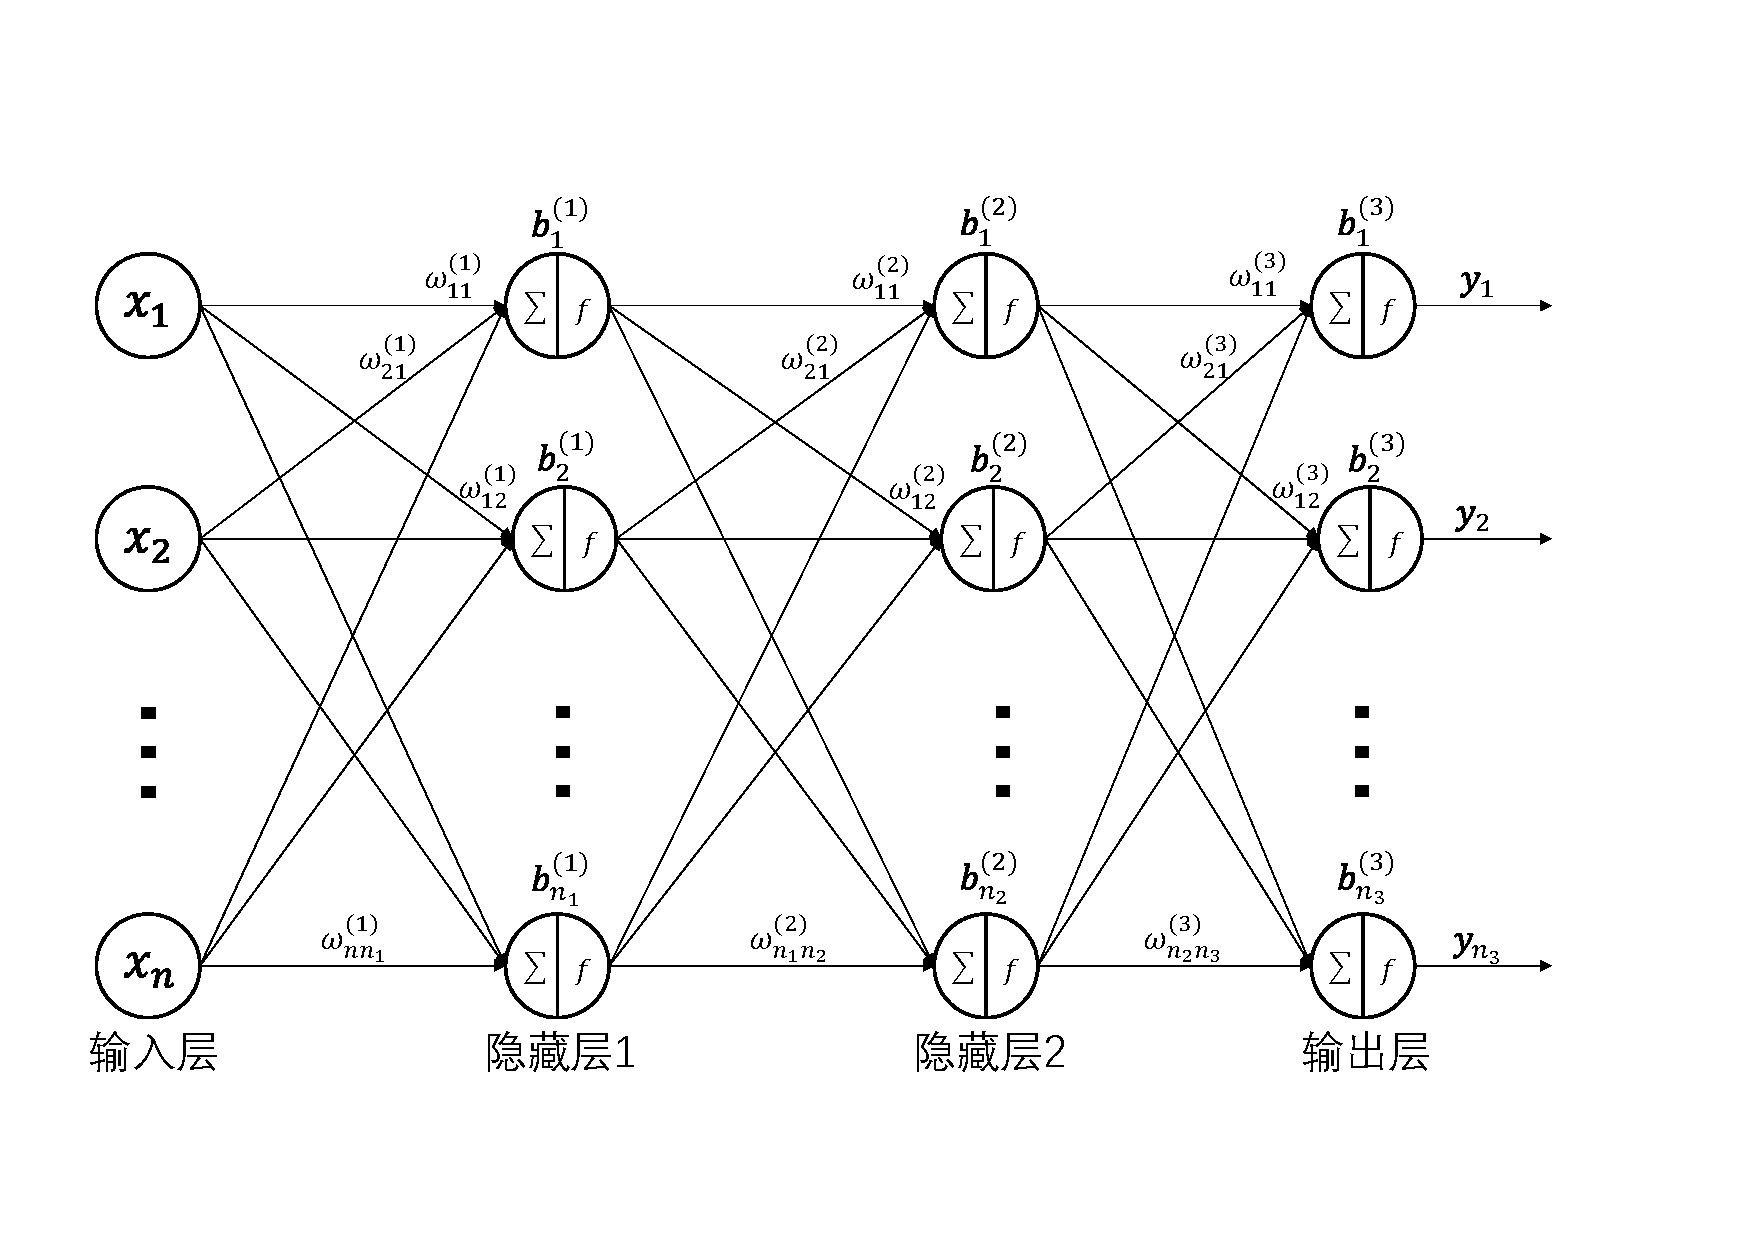
\includegraphics[width=0.9\textwidth, keepaspectratio]{figure/network.pdf}\\
	\caption{人工神经网络结构图}\label{figure:network}
\end{figure}
其中$x_i$表示各自变量的值,$n$表示自变量的个数,$n_l$表示第$l$层的神经元个数,$\omega_{ij}^{(l)}$表示第$(l-1)$层的第$i$个神经元和第$l$层的第$j$个神经元之间的连接权值,$b_j^{(l)}$表示第$l$层第$j$个神经元的偏置,$y_i$表示输出因变量的预测值,$f(\cdot)$为激活函数(Activate Function)。如果以$y_j^{(l)}$表示隐藏层$l$中的第$j$个神经元的输出,且令第$L$层为输出层,则人工神经网络的输出$y_j$由如下递推公式给出\cite{RN2}:
\begin{equation}\label{eq:神经网络公式}
	\left\{
	\begin{aligned}
		y_j       & =y_j^{(L)}                                                                & (1\leq j\leq n_L)               \\
		y_j^{(l)} & =f\left(b_j^{(l)}+\sum_{i=1}^{n_{l-1}}\omega_{ij}^{(l)}y_i^{(l-1)}\right) & (2\leq l\leq L,1\leq j\leq n_l) \\
		y_j^{(1)} & =f\left(b_j^{(1)}+\sum_{i=1}^n\omega_{ij}^{(1)}x_i\right)                 & (1\leq j\leq n)                 \\
	\end{aligned}
	\right.
\end{equation}

一个用于分类的人工神经网络输出层的激活函数通常为Logistic函数或是Softmax函数,因此基于人工神经网络的机器学习分类模型也可以看作是Logistic回归模型的推广。人工神经网络的参数由反向传播(Back propagation)算法迭代求解得出,其迭代过程表达式如下\cite{RN2}:
\begin{equation}
	\left\{
	\begin{aligned}
		\omega_{ij}^{(l)*} & =\omega_{ij}^{(l)}-\alpha E_j^{(l)}y_i^{(l-1)}                                         & (1\leq l\leq L)   \\
		E_i^{(l)}          & =\sum_{j=0}^{n_{j}}\left(E_j^{(l+1)}\omega_{ij}^{(l+1)}\right)f'\left(t_i^{(l)}\right) & (1\leq l\leq L-1) \\
		E_j^{(L)}          & =\frac{\partial E}{\partial y_j^{(L)}}f'\left(t_j^{(L)}\right)                         &
	\end{aligned}
	\right.
\end{equation}

George Cybenko曾从数学上证明:包含一个及以上隐藏层的人工神经网络可以被用来按照任意给定的精度来逼近任何连续函数,且近似精度随隐藏层神经元个数的增加而上升\cite{RN122}。这个定理表明人工神经网络是一种具有普适性的函数拟合器,这也是众多深度学习算法有效性的基础。然而在实际应用中,单纯地增加人工神经网络的深度和神经元个数会带来过拟合(Overfitting)问题。针对过拟合问题常用的解决方法有提前停止、Dropout、正则化等。
\begin{enumerate}
	\item 提前停止(Early Stopping)

	      提前停止方法的基本假设是:一个会出现过拟合的人工神经网络,其过拟合程度随训练次数的增加而增加\cite{RN134},因此为了避免过拟合,要减小训练次数,即提前停止训练。提前停止方法在训练集上进行训练时,会每隔一个固定周期计算模型在测试集上的误差,当模型在测试集上的误差比上一次训练结果差的时候,可以认为人工神经网络已经发生了过拟合,因此停止训练并使用上一次迭代结果中的参数作为模型的最终参数\cite{RN2}。

	\item Dropout

	      Dropout方法最先由Hinton于2012年提出,是一种通过阻止一个较为复杂的前馈人工神经网络中有过多神经元的共同作用来防止人工神经网络过拟合的方法\cite{RN133}。Dropout方法在人工神经网络中添加一个具有如下性质的Dropout层(设为第$l$层):
	      \begin{enumerate}[label=(\arabic*)]
		      \item Dropout层由$n_l=n_{l-1}$个单元组成;
		      \item Dropout层前向传播算法的输出为:
		            \begin{equation}
			            \begin{split}
				            y_j^{(l)}&=y_j^{(l-1)}\frac{d_j^{(l)}}{p}\\
				            d_j^{(l)}&=\left\{
				            \begin{aligned}
					            1 &  & (\mbox{概率为}p)   \\
					            0 &  & (\mbox{概率为}1-p)
				            \end{aligned}
				            \right.
			            \end{split}
		            \end{equation}
		            其中,$d_j^{(l)}$为单元的清除标记,$p$为预先指定的失活概率。
		      \item Dropout层的反向传播误差信号为:
		            \begin{equation}
			            E_j^{(l)}=E_j^{(l-1)}\frac{d_j^{(l)}}{p}
		            \end{equation}
		            其中,清除标记$d_j^{(l)}$在上一次前向传播时确定。
	      \end{enumerate}

	\item 正则化(Regularization)

	      人工神经网络的正则化分为L1正则化和L2正则化两种,都是通过修改人工神经网络的损失函数实现对人工神经网络中过大的连接权值进行抑制,进而达到使人工神经网络正则化的目的。加入L1正则化和L2正则化操作后,人工神经网络的损失函数定义如下\cite{RN2}:
	      \begin{equation}
		      E_{Regularization}=E+R(\left\{w_{ij}^{(l)}\right\})
	      \end{equation}
	      其中$E$为不加正则化时的网络损失函数,$R(\left\{w_{ij}^{(l)}\right\})$为与人工神经网络权值有关的正则化项。在L1正则化时,正则化项的表达式为:
	      \begin{equation}
		      R(\left\{w_{ij}^{(l)}\right\})=\sum_{i,j,l}|\omega_{ij}^{(l)}|
	      \end{equation}
	      即网络中所有神经元连接权值的绝对值之和;在L2正则化时,正则化项的表达式为:
	      \begin{equation}
		      R(\left\{w_{ij}^{(l)}\right\})=\sum_{i,j,l}(\omega_{ij}^{(l)})^2
	      \end{equation}
	      即网络中所有神经元连接权值的平方之和。

\end{enumerate}

\subsubsection{支持向量机}
支持向量机(Support Vector Machine,SVM)是Vapnik等人于20世纪90年代提出的一类基于监督学习(Supervised Learning)的二元线性分类器,其决策边界是对学习样本求解的最大边距超平面(Maximum-margin Hyperplane)\cite{RN90}。支持向量机基于结构风险最小化原则和核方法,能有效避免维数灾难、过拟合等问题,具有高容错性、智能化和自学习等优点\cite{RN185}。若样本空间为:
$$\mathcal{D}=\left\{(\bm x_i,y_i)|(i=1,2,\dots,n),y_i\in\left\{1,-1\right\}\right\}$$
其中$\bm x_i$为自变量,$y_i$为要预测的二元分类标记,则支持向量机的分类超平面表示为\cite{RN90}:
\begin{equation}
	\bm\omega^T\bm x+b=0
\end{equation}
其中$\bm\omega$为支持向量机的参数,该参数的确定需要保证超平面的分类间隔$\frac{2}{||\bm\omega||}$达到最大,即一个带约束的优化问题:
\begin{equation}\label{eq:基本支持向量机}
	\begin{split}
		\mathop{min}\limits_{\bm\omega,b}&\quad\frac{1}{2}||\omega||^2\\
		s.t.&\quad y_i(\bm\omega^T\bm x+b)\geq 1,i=1,2,\dots,n
	\end{split}
\end{equation}
对于错误分类的离群点,需要在式(\ref{eq:基本支持向量机})中加入松弛变量$\xi_i\geq 0$和惩罚因子$C>0$,$\xi_i$和$C$的取值分别决定了对样本分类错误的容忍程度和惩罚程度,即得到一个关于参数$\omega$的凸二次规划问题\cite{RN188}:
\begin{equation}
	\begin{split}
		\mathop{min}\limits_{\bm\omega,b}&\quad\frac{1}{2}||\omega||^2+C\sum_{i=1}^n\xi_i\\
		s.t.&\quad y_i(\bm\omega^T\bm x+b)\geq 1-\xi_i,i=1,2,\dots,n\\
		&\quad \xi_i\geq 0
	\end{split}
\end{equation}
若在当前空间不存在能很好分类的超平面,则引入核函数$k\left(\bm x\right)$,将原始输入$\bm x$映射为更高维的输入$\left(\bm x,k\left(\bm x\right)\right)$,并在新的高维空间中寻找超平面。

除上述的经典支持向量机结构之外,近年来还出现了一种改进的孪生支持向量机(Twin Support Vector Machine,TSVM)通过建立两个非平行的空间超平面,每个超平面均是离一组数据最近而离另外一组数据最远,因此能够充分利用输入训练的数据,最终为求解两个单独数据的二次规划问题,极大的提高了计算速度\cite{RN191,RN192}。

支持向量机的泛化能力和性能主要取决于核函数$k$和相关参数$\omega$的选择。支持向量机参数优化的方法主要分为直接搜索法和随机搜索法\cite{RN188}。直接搜索法主要是网格搜索法,其优点在于计算过程简单清晰、能求出全局最优解,缺点在于计算速度受网格间隔影响较大,间隔过大时不易收敛、间隔过小时速度较慢,且难以解决参数过多的问题;随机搜索法主要包括粒子群算法\cite{RN189}、遗传算法\cite{RN190}、人工免疫算法\cite{RN187}、阴阳对优化\cite{RN186}等智能算法,这些算法的普遍优点在于不受参数数目影响,计算速度快,缺点在于有可能陷入局部最优解,难以保证所求解为全局最优。

\subsubsection{K近邻分类器}\label{sec:K近邻分类器}
K近邻分类器(K nearst neighbors Classifier,KNN Classifier)算法是有监督机器学习分类中比较常用的一种基于统计的分类方法。K近邻分类器根据测试样本在特征空间中的各最近邻样本中的多数样本的类别来进行分类\cite{RN193}。假设样本空间为:
\begin{equation}
	\mathcal{D}=\left\{(\bm x_i,y_i)|(i=1,2,\dots,n),y_i\in\left\{1,-1\right\}\right\}
\end{equation}
两个例子和之间的相似度量一般采用欧氏距离表示:
\begin{equation}
	d\left(\bm x_i,\bm x_j\right)=||\bm x_i-\bm x_j||
\end{equation}
判断近邻就是使用欧氏距离测试两个例子之间的距离,距离值越小表明相似性越大,反之表明相似性越小。对于一个新样本$\bm x_{n+1}$,KNN分类器输出的类别标记$y_{m+1}$是已有样本中$d\left(\bm x_{m+1},\bm x_j\right)$最小的$k$个样本$\left\{(\bm x_i,y_i)\right\}$中数量最多的$y_j$值\cite{RN194}。

\subsubsection{贝叶斯分类器}
贝叶斯理论是处理不确定性信息的重要工具。作为一种不确定性推理方法,它基于概率和统计理论,具有坚实的数学基础,贝叶斯网络在处理不确定信息的智能化系统中已经得到了广泛的应用。贝叶斯分类器(Bayesian Classifier)是一种基于贝叶斯理论构建的分类器模型,其分类原理是通过某对象$\bm x$的先验概率,利用贝叶斯公式计算出该对象属于类别$\mathcal C_i$的后验概率$P(\bm x|\mathcal C_i)=P(\bm x\in \mathcal C_i)$,选择具有最大后验概率的类作为该对象所属的类\cite{RN199}。假设要区分的类别有$m$个,类别集合$\mathcal C=\left\{\mathcal C_i|1\leq m\leq m\right\}$,则贝叶斯分类器的分类结果表示为:
\begin{equation}
	\bm x\in \hat{\mathcal C}(\bm x)=\mathop{argmax}\limits_{\mathcal C_i\in \mathcal C}P(\mathcal C_i)P(\bm x|\mathcal C_i)
\end{equation}
目前常用的贝叶斯分类器有朴素贝叶斯分类器(Naive Bayesian Classifier,NB)和贝叶斯网分类器(Bayesian Network Classifier)两种。
\begin{enumerate}
	\item 朴素贝叶斯分类器

	      朴素贝叶斯分类器假设在给定类别$\mathcal C$的条件下,属性集$\mathcal A$中所有属性$a_i$的取值互相独立,即“朴素贝叶斯假设”\cite{RN200}:
	      \begin{equation}
		      (\forall a_i,a_j\in \mathcal A)P(a_i|\mathcal C,a_j)=P(a_i|\mathcal C)
	      \end{equation}
	      在朴素贝叶斯分类算法中,既可以独立地学习每个属性$a_i$在类别属性$\mathcal C$下的条件概率$P(a_i|\mathcal C)$,也可以独立学习每个属性 $a_i$的概率,因该值为常数,可用归一化因子$\alpha$来代替。然后,分类器应用贝叶斯公式计算特定实例数据在给定属性值下类别的后验概率\cite{RN199}\cite{RN200}\cite{RN201}:
	      \begin{equation}
		      P(\mathcal C|a_1,a_2,\cdots)=\alpha P(\mathcal C)\prod_{a_i\in\mathcal A}P(a_i|\mathcal C)
	      \end{equation}
	      并预测该实例属于后验概率最大的类别。

	\item 贝叶斯网络分类器

	      贝叶斯网络通过提供图形化的方法来表示知识,是一个有向无环图,其中结点代表论域中的变量,有向弧代表变量的关系,条件概率表示变量之间影响的程度,通过贝叶斯网络可以清楚地反映实际应用中变量之间的依赖关系。在贝叶斯网络中,后验概率表达式为\cite{RN198}:
	      \begin{equation}
		      P(\mathcal C_i|\bm x)=\frac{P(\mathcal C_i)\prod_{(\bm x_j,y_j)\in\mathcal D}P(\bm x_j|\mathcal C_i,\pi(\bm x_j))}{P(\bm x)}
	      \end{equation}
	      其中$\pi(\bm x_j)$表示结点$\bm x_j$除类别结点$\mathcal C_i$之外的所有父结点。
\end{enumerate}

贝叶斯分类器是各种分类器中分类错误概率最小或者在预先给定代价的情况下平均风险最小的分类器。其优点是具有很强的学习和推理能力,能够很好地利用先验知识,缺点是对发生频率较低的事件预测效果不好,且推理与学习过程是一个NP难问题。

\subsubsection{决策树}
决策树(Decision Tree)是在已知各种情况发生概率的基础上,通过构成决策树来求取净现值的期望值大于等于零的概率,是直观运用概率分析的一种图解法。它利用树的结构将数据记录进行分类,树的一个叶结点就代表某个条件下的一个记录集,根据记录字段的不同取值建立树的分支;在每个分支子集中重复建立下层结点和分支,便可生成一棵决策树\cite{RN195}。

决策树的构造过程一般分为3个步骤:
\begin{enumerate}
	\item 特征选择

	      从众多的特征中选择一个特征作为当前节点分裂的标准,特征选择有不同的量化评估方法,产生的决策树也有所不同,常见的决策树特征选择算法有通过最大化信息增益选择特征的ID3方法\cite{quinlan1986induction}、通过最大化信息增益比选择特征的C4.5方法\cite{quinlan2014c4}以及通过最小化Gini指数选择特征的CART方法\cite{breiman2017classification}等。特征选择的准则是在使用某特征对数据集划分之后,各数据子集的纯度要比划分前的数据集D的纯度高,即使得分类后各类别子集的元素尽可能的相似。

	\item 决策树的生成

	      根据选择的特征评估标准,从上至下递归地生成子节点,直到数据集不可分则停止决策树停止生长。这个过程实际上就是使用满足划分准则的特征不断的将数据集划分成纯度更高,不确定行更小的子集的过程。

	      %\item 决策树的裁剪:决策树容易过拟合,一般需要剪枝来缩小树结构规模、缓解过拟合。

\end{enumerate}

具体来说,决策树的构建方法可以表示为算法\ref{alg:DT}\cite{RN90}。
\begin{algorithm}[htbp]
	\caption{\mycaptionfont 决策树学习的基本算法}
	\label{alg:DT}
	\begin{algorithmic}[1]
		\Require 训练集$\mathcal{D}=\left\{(\bm x_i,y_i)|1\leq i\leq m\right\}$、属性集$\mathcal{A}=\left\{a_i|1\leq i\leq d\right\}$
		\Ensure $\forall (\bm x_i,y_i)\in \mathcal{D}$,属性值$a_i(\bm x_i)$存在
		\Function {DecisionTree}{$\mathcal{D}$,$\mathcal{A}$}
		\If{$\mathcal{D}$中的样本全部属于同一类别$C$}
		\State \Return 单节点树,类别标记为$C$
		\EndIf
		\If{$\mathcal{A}=\varnothing$}
		\State \Return 单节点树,类别标记为$\mathcal{D}$中样本数最多的类
		\EndIf
		\State 计算$\mathcal{A}$中每个特征的信息增益(ID3算法)或信息增益比(C4.5算法),从中选择最优属性$a_{best}$
		\For{$a_{best}$的每一可能值$a_{best}^t$}
		\State 令$\mathcal{D}'=\left\{(\bm x_i,y_i)|a_{best}(\bm x_i,y_i)=a_{best}^t,(\bm x_i,y_i)\in \mathcal{D}\right\}$
		\If{$\mathcal{D}'=\varnothing$}
		\State 添加叶节点,类别标记为$\mathcal{D}$中样本数最多的类
		\Else
		\State 递归添加分支节点\Call{DecisionTree}{$\mathcal{D}'$,$\mathcal{A}$}
		\EndIf
		\EndFor
		\EndFunction
	\end{algorithmic}
\end{algorithm}

假定没离散属性$a_i$都有各$V_i$个可能取值$\mathcal A_i=\left\{a_i^t|1\leq t\leq V_i\right\}$,令样本集$\mathcal D_i^t=\left\{(\bm x_i,y_i)|a_i(\bm x_i)=a_i^t\right\}$。则在CART决策树中,选择最优属性的标准为Gini指数的最小值\cite{RN90}:
\begin{equation}
	\begin{split}
		Gini\_index(\mathcal{D},a_i)&=\sum_{t=1}^{V_i}\frac{|\mathcal D_i^t|}{|\mathcal{D}|}Gini(\mathcal D_i^t)\\
		Gini(\mathcal{D})&=1-\sum_{(\bm x_i,y_i)\in \mathcal{D}}p(x_i|\mathcal{D})^2\\
	\end{split}
\end{equation}
在ID3算法中,选择最优属性的标准为信息增益$Gain(\mathcal{D},a_i)$的最大值\cite{RN90}:
\begin{equation}
	\begin{split}
		Gain(\mathcal{D},a_i)&=H(\mathcal{D})+H(\mathcal{D}|a_i)\\
		H(\mathcal{D})&=-\sum_{(\bm x_i,y_i)\in \mathcal{D}}p(x_i|\mathcal{D}) log_{2}p(x_i|\mathcal{D})\\
		H(\mathcal{D}|a_i)&=-\sum_{t=1}^{V_i}\frac{|\mathcal D_i^t|}{|\mathcal{D}|}H(\mathcal D_i^t)
	\end{split}
\end{equation}
但是最大化信息增益的方法会有选择取值较多的特征的倾向,因此在C4.5算法中对最优属性的选择方法进行改进,产生了最大化信息增益比的方法。信息增益比$GainRatio(\mathcal{D},a_i)$的表达式为\cite{RN90}:
\begin{equation}
	GainRatio(\mathcal{D},a_i)=\frac{Gain(\mathcal{D},a_i)}{H(\mathcal{D})}
\end{equation}
不论是最大化信息增益还是最大化信息增益比,其目的都是通过计算子集特征的不确定性,使得依据特征划分得到的子集纯度尽可能高。另外,

%\iffalse
\subsection{分类预测模型的改进方法:集成学习}
集成学习(ensemble learning)技术是指利用基学习器(Basic Learning Machine)的多个版本来解决同一个问题,并使用某种规则将各个学习器的结果进行整合,从而获得比单个学习器效果更好的准确率和泛化能力的一种方法。集成学习可以用于分类问题,回归问题,特征选取,异常点检测等的集成。在用于分类的集成学习方法中,基学习器又被称为弱分类器(Weak Classifier),其仅能对少量样本进行正确分类,而用于分类的集成学习则是通过组合多个弱分类器形成一个具有较高准确率的强分类器(Strong Classifier)的过程。目前主流的集成学习方法主要有三种\cite{RN90}\cite{RN197}:

\begin{enumerate}
	\item Stacking

	      Stacking的基本思想是训练一系列弱分类器,然后使用另一个分类器来组合这些弱分类器预测结果。Stacking首先将训练集$\mathcal D$分为两个不相交的训练集$\mathcal D_1$和$\mathcal D_2$,在$\mathcal D_1$上训练一系列分类器$f_1(\cdot),f_2(\cdot),f_3(\cdot),\dots$,然后用这一系列分类器在$\mathcal D_2$上的分类结果和$\mathcal D_2$中的分类标签再构造一个训练集:
	      $$\mathcal D_3=\left\{\left(f_1(\bm x),f_2(\bm x),f_3(\bm x),\dots,y\right)|(\bm x,y)\in\mathcal D_2\right\}$$
	      最后使用$\mathcal D_3$训练分类器$g(\cdot)$。Stacking算法的分类结果由下式给出:
	      $$\hat y=g(f_1(\bm x),f_2(\bm x),f_3(\bm x),\dots)$$

	\item Bagging

	      Bagging全称Bootstrap Aggregating,又称引导聚合法。Bagging通过对原训练集$\mathcal D$进行有放回的采样,构建出大小相同的多个新训练集$\mathcal D_1,\mathcal D_2,\mathcal D_3,\dots$,然后用这些新的训练集训练出多个弱分类器$f_1(\cdot),f_2(\cdot),f_3(\cdot),\dots$。对于某个样本$\bm x$,Bagging统计这些弱分类器各自的分类结果$f_1(\bm x),f_2(\bm x),f_3(\bm x),\dots$,以投票的形式来决定最终分类结果。Bagging集成学习的代表性算法是随机森林算法(Random Forest),它以决策树作为Bagging的基学习器。

	\item Boosting

	      Boosting是一个迭代的过程,每次迭代都会生成一个新的训练集$\mathcal D_t$,并用$\mathcal D_t$训练出一个新的分类器$f_t(\cdot)$,最终的分类器由各个迭代过程中训练出的分类器$f_1(\cdot),f_2(\cdot),f_3(\cdot),\dots$进行加权组成。Boosting生成新训练集的方法为:假设在第$t$次迭代时,将训练好的分类器$f_t(\cdot)$分类错误的训练数据组成集合$\mathcal D_t^{e}$、分类正确的训练数据组成集合$\mathcal D_t^{c}$,则在下一次迭代时,新训练集$\mathcal D_{t+1}$是在$\mathcal D_t$中提高样本$\bm x^e\in \mathcal D_t^{e}$的权重、降低样本$\bm x^c\in \mathcal D_t^{c}$的权重而来。

\end{enumerate}
%\fi

\subsection{分类预测模型的评价指标}
\subsubsection{分类正确率和混淆矩阵}
如果要对一个分类器$f(\cdot)$的准确性进行评价,分类正确率是最简单直观的方法。假设测试集为$\mathcal D=\left\{(\bm x_i,y_i)|1\leq i\leq m\right\}$,分类器的分类正确率$Accuracy$表示分类器在测试集$\mathcal D$上预测正确的样本个数占测试集总样本数的比值。其计算式为:
\begin{equation}
	Accuracy=\frac{|\left\{(\bm x,y)|(\bm x,y)\in\mathcal D,f(\bm x)=y\right\}|}{|\mathcal D|}
\end{equation}

分类正确率基本可以反映一个分类器的准确性,但是不能反映样本分类的具体情况。对于在测试集上进行的一次分类器评价,分类器对样本的处理结果可以分为以下4类:
\begin{enumerate}
	\item TP(True Positive)真正类:分类器将正样本判断为正样本,分类正确;
	\item FN(False Negative)假负类:分类器将正样本错判为负样本,统计学上称为第一类错误(Type I Error);
	\item FP(False Positive)假正类:分类器将负样本错判为正样本,统计学上称为第二类错误(Type II Error);
	\item TN(True Negative)真负类:分类器将负样本判断为负样本,分类正确。
\end{enumerate}
将这4个分类结果占测试集总量的比率共同呈现于表\ref{tab:混淆矩阵}中,所形成的2$\times$2矩阵就称为混淆矩阵(Confusion Matrix)。相比于分类正确率,混淆矩阵能反映有关分类器性能的更加具体的信息,是分类预测模型性能评价的常用指标。
\begin{table}[htbp]
	\setstretch{1.5}
	\centering
	\caption{混淆矩阵}
	\begin{tabular}{|c|c|c|}
		\hline
		\diagbox{预测值}{混淆矩阵}{真实值} & 正 & 负 \\
		\hline
		正                                 & TP & FP \\
		\hline
		负                                 & FN & TN \\
		\hline
	\end{tabular}
	\label{tab:混淆矩阵}
\end{table}

\subsubsection{ROC曲线和AUC值}
ROC全称Receiver Operating Characteristic,中文直译接收者操作特征,ROC曲线上每个点反映着对同一信号刺激的感受性,是一种针对于输出值为类别概率的分类器的评价指标。ROC曲线评价分类器的性能基于以下三个指标:
\begin{enumerate}
	\item TPR(True Postive Rate)真正类率:$TPR=TP/(TP+FN)$,又称分类器的灵敏度(Sensitivity),代表正类中被分类器预测预测正确的比例。
	\item TNR(True Negative Rate)真负类率:$TNR=TN/(FP+TN)=1-TPR$,又称分类器的特异性(Specificity),代表负类中被分类器预测预测正确的比例。
	\item FPR(False Postive Rate)假正类率:$FPR=FP/(FP+TN)$,代表负类中被分类器预测预测错误的比例。
\end{enumerate}
对于一个输出值为正类概率$p$的二分类器,分别选择不同的阈值(threshold)$t$作为判断类别的标准,使得预测值$\hat y$满足:
\begin{equation}
	\hat y=\left\{
	\begin{split}
		\text{正类}&\quad&p\geq t\\
		\text{负类}&\quad&p<t
	\end{split}
	\right.
\end{equation}
对于每个分类结果,都分别计算其TPR和FPR值,以FPR为横轴坐标,TPR为纵轴坐标绘制出的曲线即为ROC曲线。而AUC值(Area under Curve)就是ROC曲线下的面积,介于0$\sim$1之间。AUC值越接近1,表明ROC曲线越接近FPR-TPR平面上的(0,1)点,分类器的特异性和灵敏度越高,分类效果越好。

\subsection{本实验所使用的主要数据分析平台介绍}
\subsubsection{Python}
Python是一种计算机程序设计语言。是一种面向对象的动态类型语言,因其简洁易学和类库丰富的特征而成为当前数据分析领域最流行的语言之一。

本实验所使用的Python库有:pandas、sklearn、pytorch、seaborn、matplotlib、numpy、impyute

\subsubsection{Pandas}
Pandas(Python Panel Data Analysis Library)是一种基于Python语言和NumPy科学计算库的数据分析工具。Pandas纳入了大量数据分析库和一些标准的数据模型,提供了高效地操作大型数据集所需的工具,提供了大量能使用户快速便捷地处理数据的函数和方法。

\subsubsection{Scikit-Learn}
Scikit-learn(sklearn)是基于Python语言和NumPy构建的针对机器学习应用的数据挖掘和数据分析工具,也是机器学习中常用的第三方模块,对常用的机器学习方法进行了封装,包括回归(Regression)、降维(Dimensionality Reduction)、分类(Classfication)、聚类(Clustering)等方法。

\subsection{R语言}
R是一套由数据操作、计算和图形展示功能整合而成的套件。包括:有效的数据存储和处理功能、完整的数组计算操作符、拥有完整体系的数据分析工具、为数据分析和显示提供的强大图形功能以及一套简洁易学的编程语言。R是属于GNU系统的一个自由、免费、源代码开放的软件,它是一个用于统计计算和统计制图的优秀工具。

本实验所使用的R语言程序包有:mice、VIM

\subsection{Matlab}
MATLAB是美国MathWorks公司出品的商业数学软件,用于算法开发、数据可视化、数据分析以及数值计算的高级技术计算语言和交互式环境,它在数学类科技应用软件中在数值计算方面首屈一指。MATLAB可以进行矩阵运算、绘制函数和数据、实现算法、创建用户界面、连接其他编程语言的程序等,主要应用于工程计算、控制设计、信号处理与通讯、图像处理、金融分析等领域,其内置有许多简洁高效的数据分析方法。


\section{实验设计}
\subsection{数据预处理}\label{sec:数据预处理}
由于本实验所用的Pima印第安人糖尿病数据集是来自美国国家糖尿病与消化及肾脏疾病研究所的权威数据集,因此假定数据集中的无缺失数据全部正确,在数据预处理阶段仅对数据集中的数据缺失进行处理。预处理前先使用Excel统计原数据集中正例(“Outcome”列为1的数据点)和负例(“Outcome”列为0的数据点)比例,得到正例个数为268,负例个数为500。

\subsubsection{确定缺失项}\label{sec:确定缺失项}
首先绘制各特征间的关系散点图,从图中找出存在异常数据的属性。调用Seaborn库的pairplot函数对数据集各特征间的关系散点图矩阵进行绘制,结果如图\ref{figure:交叉图}。图中对角线上的图像表示某个变量在各个值域上的样本数量,非对角线上的图像为数据集中两个变量间取值关系的散点图,其中蓝色数据点中“Outcome”取值为1,即患有糖尿病;橙色数据点中“Outcome”取值为0,即不患有糖尿病。
\begin{figure}[htbp]
	\centering
	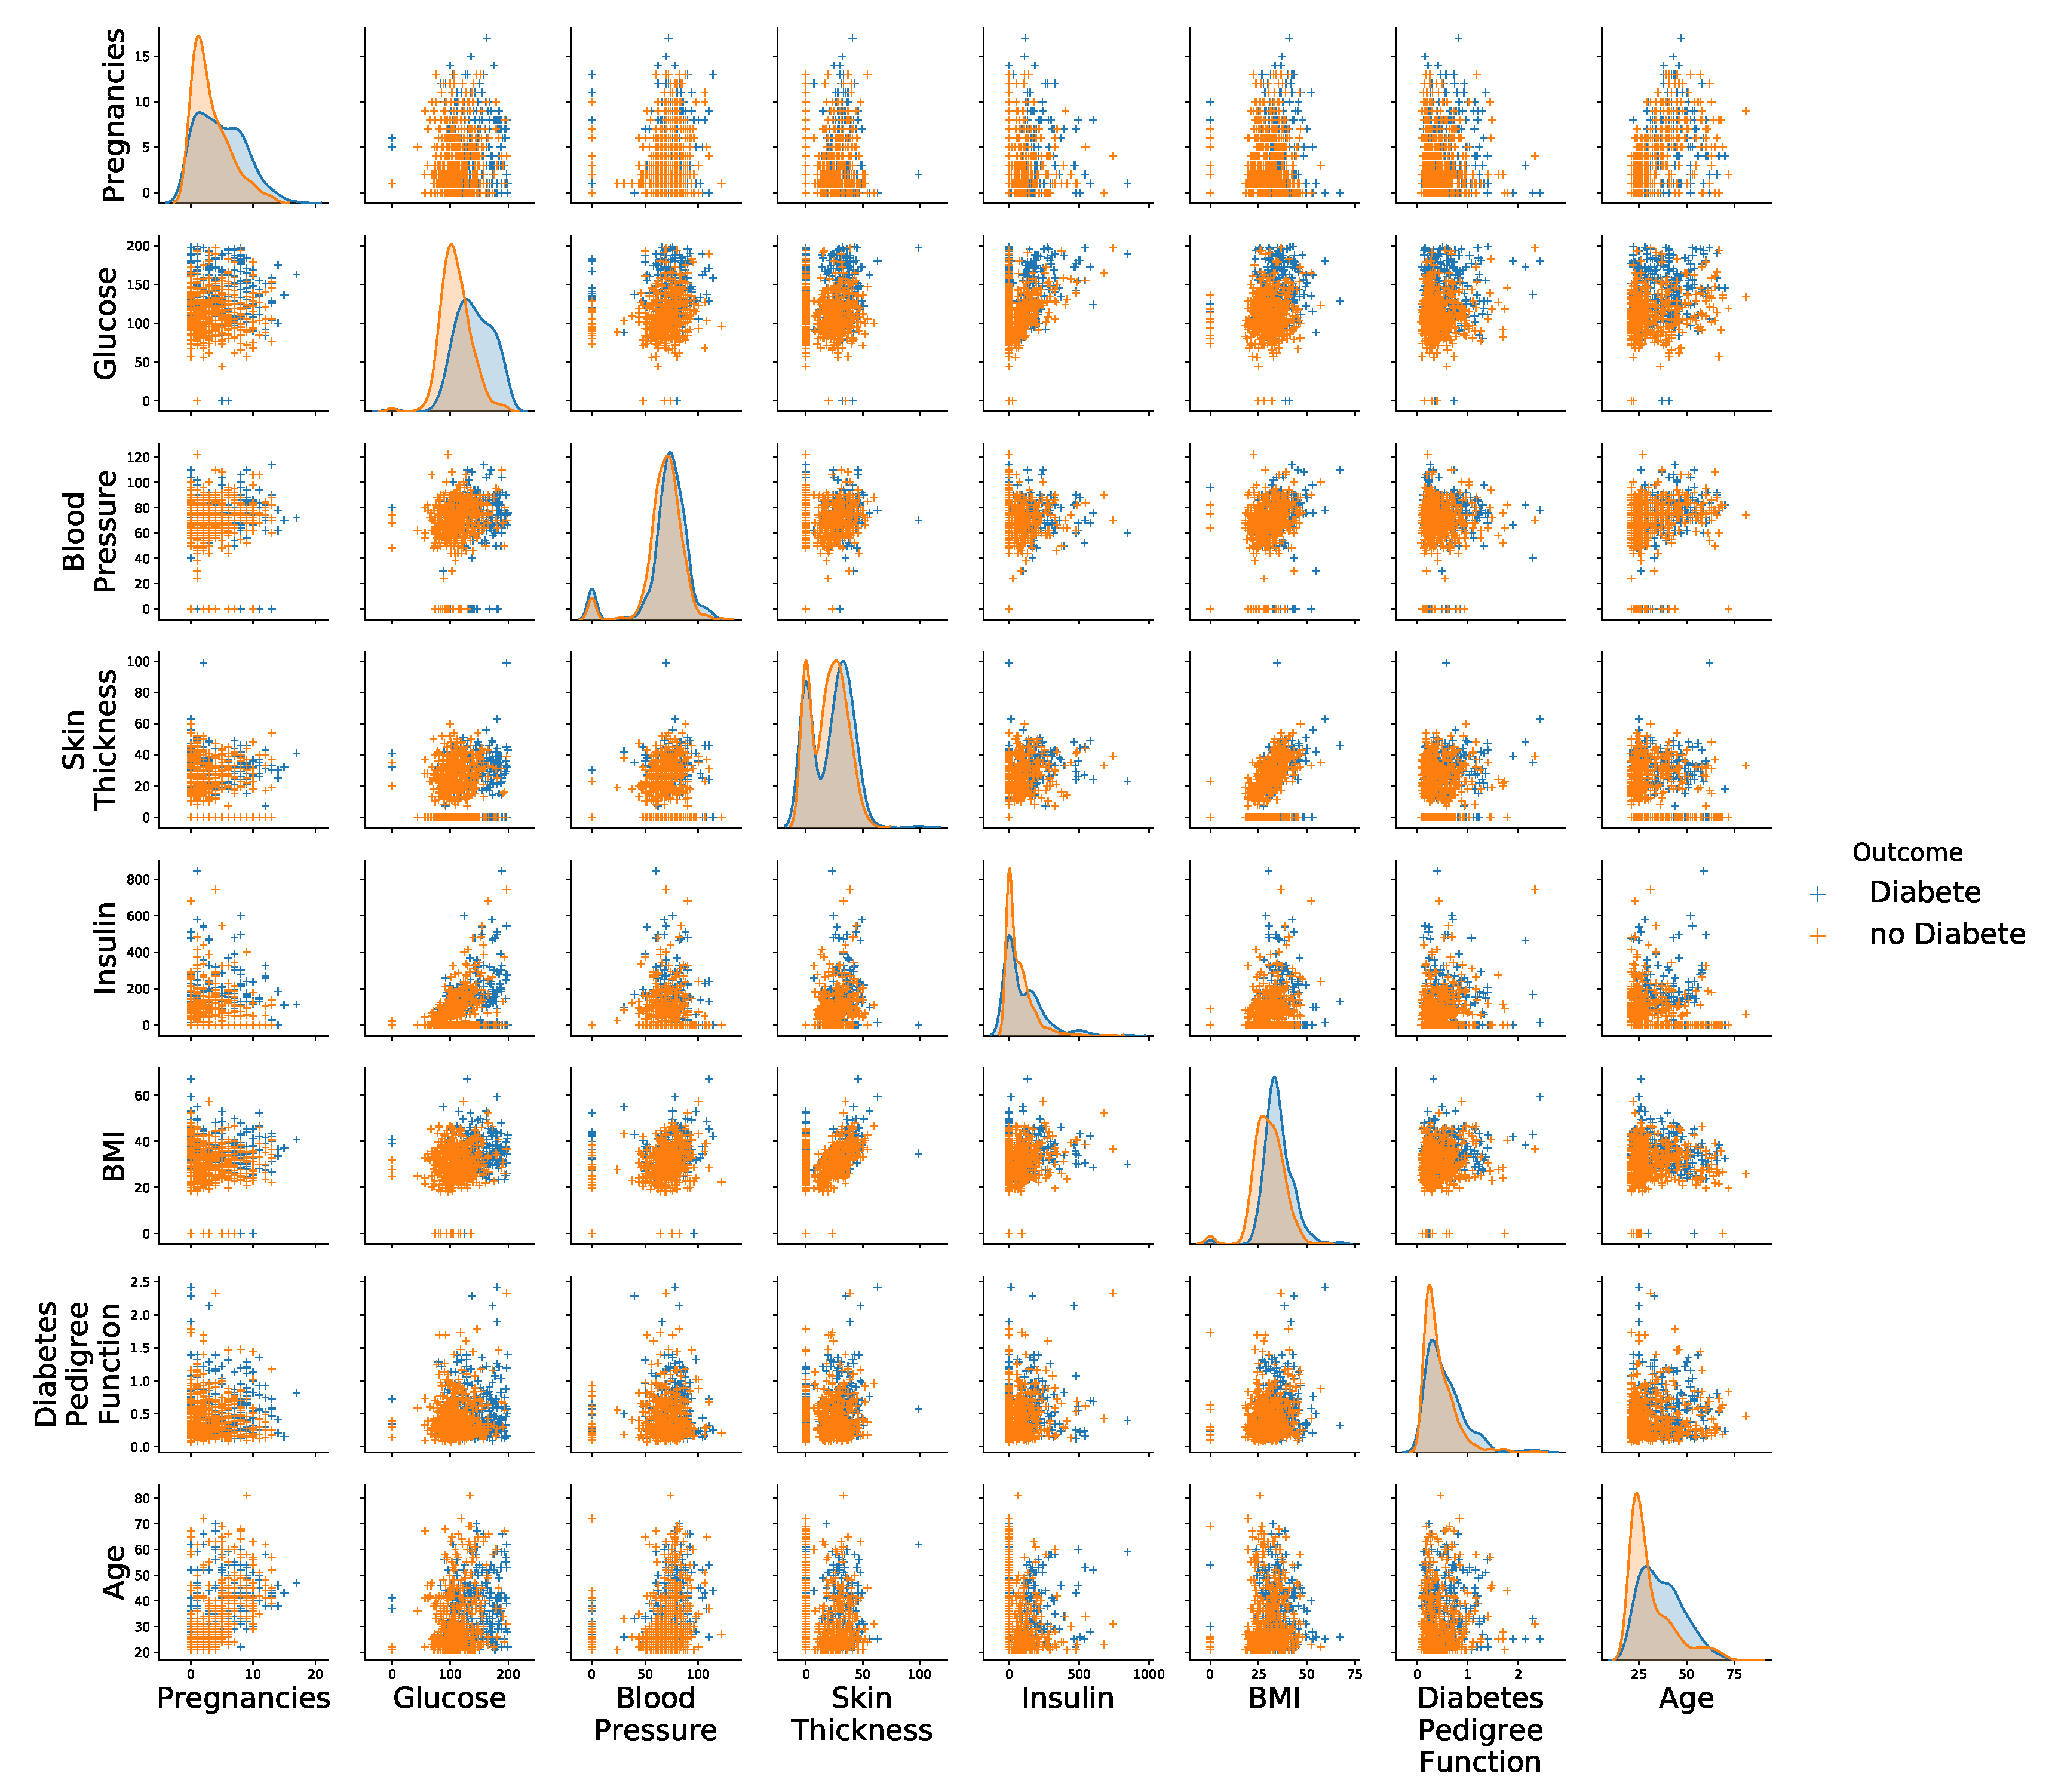
\includegraphics[width=\textwidth]{figure/1.pdf}
	\caption{各特征间的关系散点图矩阵}
	\label{figure:交叉图}
\end{figure}
从图中可以看出,有少量数据点的“Glucose”和“BMI”属性偏离数据集总体而取值为0,有很多数据点的“BloodPressure”、“SkinThickness”、“Insulin”取值为0。但是经查阅资料\cite{bmi}\cite{ins}可知,人体内的葡萄糖含量(Glucose)、身体质量指数(BMI)、体内胰岛素含量(Insulin)都不可能为0,而血压(BloodPressure)和皮肤厚度(SkinThickness)显然也都不可能取0值。因此这些异常数据不能看作是属性取值空间的一部分,需要作为MCAR或MAR缺失进行处理。

使用Python中的Pandas分析框架读取原始数据集“diabetes.txt”,将数据集中“Glucose”、“BMI”、“BloodPressure”、“SkinThickness”、“Insulin”这五项属性下的0值全部置为NaN,保存为逗号表达式文件“diabetes.csv”,进行进一步的缺失数据处理。

\subsubsection{确定缺失项处理方法}\label{sec:确定缺失项处理方法}
缺失属性项确定之后,接下来就需要确定各缺失项的处理方法。
首先使用R语言读取“diabetes.csv”的数据并对数据集中的数据缺失情况进行统计:
\begin{enumerate}
	\item 统计“diabetes.csv”中的数据总行数,得到结果768;
	\item 使用mice包中的md.pattern()函数统计数据集中的数据缺失情况,数据缺失情况统计表(表\ref{tab:缺失数据统计})。
\end{enumerate}
\begin{table}[htbp]
	\setstretch{1.5}
	\centering
	\caption{数据缺失情况}
	\begin{tabular}{|c|ccccc|}
		\hline
		\diagbox{数据点数量}{是否缺失}{列名} & Glucose & BMI & BloodPressure & SkinThickness & Insulin \\\hline
		392                                  & 否      & 否  & 否            & 否            & 否      \\
		1                                    & 是      & 否  & 否            & 否            & 否      \\
		140                                  & 否      & 否  & 否            & 否            & 是      \\
		1                                    & 否      & 是  & 否            & 否            & 否      \\
		4                                    & 是      & 否  & 否            & 否            & 是      \\
		2                                    & 否      & 否  & 是            & 否            & 是      \\
		192                                  & 否      & 否  & 否            & 是            & 是      \\
		1                                    & 否      & 是  & 否            & 否            & 是      \\
		26                                   & 否      & 否  & 是            & 是            & 是      \\
		2                                    & 否      & 是  & 否            & 是            & 是      \\
		7                                    & 否      & 是  & 是            & 是            & 是      \\\hline
		列缺失总量                           & 5       & 11  & 35            & 227           & 374     \\\hline
	\end{tabular}
	\label{tab:缺失数据统计}
\end{table}
统计结果显示,数据集中有392个数据点没有数据缺失,有140个数据点只缺失“Insulin”数据、192个数据点缺失“Insulin”和“SkinThickness”数据;“Insulin”列缺失了374个数据,“SkinThickness”列缺失了227个数据。因此可以看出数据缺失主要集中在“Insulin”和“SkinThickness”两列,在数据预处理中应考虑删除。

由\ref{subsec:划分训练集和测试集时的填补方法}节的分析可知,当数据划分训练集和测试集时,训练集和测试集要分开填补,且对测试集进行填补时不能包含分类标签信息。为简单起见,本实验对测试集只执行删除操作,不进行填补操作;而对训练集,除尝试删除数据外,本实验还将使用\ref{subsec:单值填补}节中介绍的K近邻填补法、EM填补法、以及\ref{subsec:多重填补}节介绍的多重回归中的PMM方法和MICE方法对数据集进行填补,形成多个训练集供后续的分类器训练。

\subsubsection{确定数据集的划分方法}\label{sec:确定数据集的划分方法}
按照实验指导上不改变数据集顺序的要求,为保证数据量足够以及训练集和测试集大小的均衡,本文将把数据集的划分放在数据删除之后,使得删除和划分后的数据集满足以下要求:
\begin{enumerate}
	\item 删除和划分操作前后数据的相对顺序不发生变化;
	\item 划分出的训练集和测试集之间的数据数量之比为6:4;
	\item 能最大限度地利用表中的全部数据
\end{enumerate}
按照后续操作的不同,数据集的删除和划分可以分为两种情况处理:
\begin{enumerate}
	\item 划分后不进行数据填补

	      当划分之后没有数据填补操作时,删除完成后的数据集中不应该包含缺失数据,即在删除阶段删掉所有的有缺失数据点,此时只需要按照前60\%为训练集,后40\%为测试集的规则对删除后的数据集进行划分即可。

	\item 划分后要进行数据填补

	      当划分后还要进行数据填补时,划分后填补前的训练集中应包含一部分缺失数据,因此为保证划分后的数据满足上述的三条要求,可以从数据集$\mathcal D$的最后一个数据点$d_M$开始向前搜索,逐步剔除有缺失的数据,直到在某个数据点$d_n$处,有:
	      \begin{equation}\label{eq:划分1}
		      n:|\left\{d_i|n\leq i\leq M,d_i\in\mathcal D,d_i\text{无缺失}\right\}|=6:4
	      \end{equation}
	      此时的n即为训练集$\mathcal D_{train}$和测试集$\mathcal D_{test}$的分界点:
	      \begin{equation}\label{eq:划分2}
		      \begin{split}
			      \mathcal D_{train}&=\left\{d_i|1\leq i< M,d_i\in\mathcal D\right\}\\
			      \mathcal D_{test}&=\left\{d_i|n\leq i\leq M,d_i\in\mathcal D,d_i\text{无缺失}\right\}
		      \end{split}
	      \end{equation}
	      可以证明,依照式(\ref{eq:划分1})和式(\ref{eq:划分2})划分完成后的训练集$\mathcal D_{train}$和测试集$\mathcal D_{test}$满足前面列出的三个条件,且划分后的训练集$\mathcal D_{train}$中包含缺失数据而测试集$\mathcal D_{test}$不包含缺失数据。
\end{enumerate}

\subsubsection{进行数据集的删除和划分}\label{sec:进行数据集的删除和划分}
\begin{enumerate}
	\item 划分后不进行数据填补

	      由\ref{sec:确定缺失项处理方法}节的分析可知,数据缺失大量集中于“Insulin”和“SkinThickness”两列,因此可以先删除其中的一列或两列,再删除含缺失数据的数据点。但是如果考虑到实际中胰岛素对糖尿病的重要影响,数据缺失最多的“Insulin”列反而是最不应该删除的列。考虑到实验的全面性,本文将尝试以下4种删除方法,并按照\ref{sec:确定数据集的划分方法}节介绍的不进行数据填补的划分方法生成4个训练集和4个测试集:
	      \begin{enumerate}[label=(\arabic*)]
		      \item 保留所有列,只删除缺失数据点,形成训练集“train\_drop.csv”和测试集“test\_drop.csv”;
		      \item 只删除“Insulin”列,再删除缺失数据点,形成训练集“train\_dropI.csv”和测试集“test\_dropI.csv”;
		      \item 只删除“SkinThickness”列,再删除缺失数据点,形成训练集“train\_dropS.csv”和测试集“test\_dropS.csv”;
		      \item 将“Insulin”和“SkinThickness”一起删除,再删除缺失数据点,形成训练集“train\_dropIS.csv”和测试集“test\_dropIS.csv”。
	      \end{enumerate}

	\item 划分后要进行数据填补

	      针对要进行后续的数据填补的删除和划分,只需要按照按照\ref{sec:确定数据集的划分方法}节介绍的划分方法生成一个含有缺失数据的训练集“train\_impute\_no.csv”和一个无缺失数据的测试集“test\_impute.csv”即可。

\end{enumerate}

\subsubsection{进行数据集的规范化}\label{sec:进行数据集的规范化}
由\ref{subsec:划分训练集和测试集时的填补方法}节的分析可知,对训练集进行的数据预处理不能使用到测试集的信息,因此在进行数据规范化时,不能将训练集和测试集放在一起进行规范化。为简单起见,假定数据缺失为MCAR缺失,即缺失数据和完备数据有相似分布,选用\ref{sec:数据规范化}节中介绍的零-均值规范化方法,使用\ref{sec:进行数据集的删除和划分}中生成的各训练集的均值和方差对训练集自身以及对应的测试集分别进行规范化。

使用pandas读取\ref{sec:进行数据集的删除和划分}中生成的5对训练测试集,计算训练集中非NaN数据的均值和方差,按照公式(\ref{eq:Z-score标准化公式})对训练集和对应的测试集中除“Outcome”列外的非NaN数据进行规范化。规范化完成后分别保存为训练集文件和测试集文件:
\begin{enumerate}
	\item “train\_drop.csv”、“test\_drop.csv”$\rightarrow$“train\_norm.csv”、“test\_norm.csv”;
	\item “train\_dropI.csv”、“test\_dropI.csv”$\rightarrow$“train\_normI.csv”、“test\_normI.csv”;
	\item “train\_dropS.csv”、“test\_dropS.csv”$\rightarrow$“train\_normS.csv”、“test\_normS.csv”;
	\item “train\_dropIS.csv”、“test\_dropIS.csv”$\rightarrow$“train\_normIS.csv”、“test\_normIS.csv”;
	\item “train\_impute\_no.csv”、“test\_impute.csv”$\rightarrow$“train\_norm\_impute\_no.csv”、

	      “test\_norm\_impute.csv”。
\end{enumerate}
其中,前4个数据集能直接用于分类模型训练和测试,最后一个数据集需要对训练集进行填补后才能用于分类模型训练和测试。

\subsubsection{填补缺失项}\label{sec:填补缺失项}
对缺失项填补主要针对\ref{sec:进行数据集的规范化}节中得到的训练集“train\_norm\_impute\_no.csv”。填补采用下列四种方式进行,共得到4个新的训练集:
\begin{enumerate}

	\item K近邻填补

	      使用Matlab的importdata()函数读取“train\_norm\_impute\_no.csv”,并使用K近邻填补函数knnimpute()对数据集进行填补,选择参数$k=5$,将填补得到的数据集保存到“train\_impute\_knn.csv”文件中;

	\item EM填补

	      使用pandas读取“train\_norm\_impute\_no.csv”,并使用impyute中的EM函数imputation.cs.em对数据进行EM填补,填补结果保存到“train\_impute\_em.csv”中。

	\item 预测均值匹配填补

	      使用R语言读取“train\_norm\_impute\_no.csv”,并使用mice包中的mice()函数、设置meth参数为“PMM”对数据进行预测均值匹配填补,得到的无缺失数据集保存到“train\_impute\_pmm.csv”文件中;

	\item MICE填补

	      使用pandas读取“train\_norm\_impute\_no.csv”,并使用impyute中的函数imputation.cs.mice对数据进行mice填补,填补结果保存到“train\_impute\_mice.csv”中。

\end{enumerate}

\subsection{进行分类学习}
经过\ref{sec:数据预处理}节中的操作总共可以得到8个训练集和5个测试集,它们的对应关系如表\ref{tab:tt对应关系}。在使用这些数据集对分类模型和填补效果进行测试时,所用的训练集和测试集必须严格对应。为简单起见,在下文中以数据集的预处理方式指代使用了某个训练集进行训练并使用了对应的测试集进行测试。
\begin{table}[htbp]
	\setstretch{1.5}
	\centering
	\caption{训练集和测试集的对应关系}\label{tab:数据集表}
	\begin{tabular}{|c|c|c|}
		\hline
		训练集                  & 测试集                 & 预处理方式                 \\
		\hline
		train\_norm.csv         & test\_norm.csv         & 删除数据点                 \\
		\hline
		train\_normI.csv        & test\_normI.csv        & 删除Insulin                \\
		\hline
		train\_normS.csv        & test\_normS.csv        & 删除SkinThickness          \\
		\hline
		train\_normIS.csv       & test\_normIS.csv       & 删除Insulin和SkinThickness \\
		\hline
		train\_impute\_knn.csv  & test\_norm\_impute.csv & KNN填补                    \\
		\hline
		train\_impute\_em.csv   & test\_norm\_impute.csv & EM填补                     \\
		\hline
		train\_impute\_pmm.csv  & test\_norm\_impute.csv & PMM填补                    \\
		\hline
		train\_impute\_mice.csv & test\_norm\_impute.csv & MICE填补                   \\
		\hline
	\end{tabular}
	\label{tab:tt对应关系}
\end{table}

\subsubsection{逻辑回归}\label{sec:进行逻辑回归}
由公式\ref{eq:逻辑回归公式}和公式\ref{eq:神经网络公式}可知,逻辑回归模型相当于一个无隐藏层、单输出的Sigmoid神经网络,因此可以使用Pytorch中构造神经网络的方法构造逻辑回归模型,其结构和参数如下:
\begin{itemize}
	\item 结构:无隐藏层、多输入、单输出、激活函数为Sigmoid的神经网络;
	\item 参数调节算法:学习率为0.35的Adagrad算法;
	\item 损失函数:模型输出值(输入为正样本的概率)和样本“Outcome”列值(样本类别的01标记)间的均方误差(MSELoss)。
\end{itemize}

除上述参数之外,逻辑回归模型还需要确定输出的类别判定阈值。由\ref{subsec:划分训练集和测试集时的填补方法}节的分析可知,使用测试集调整判定阈值会使得模型中包含测试集的样本分布信息而导致测试结果产生偏颇,因此只能使用训练集进行阈值调整。这里采用平衡假正例(FP)和假负例(FN)样本的方法,即:调整输出类别判定阈值,使得在训练完成后,分类器对训练集的分类结果中的假正例和假负例样本数量大致相同,按照此方法,分别在表\ref{tab:数据集表}中的8个训练集上各训练一个逻辑回归模型,使用不同阈值判定这些模型在各自训练集上的输出,找出使假正例和假负例样本数量比较接近的判定阈值,得到的判定阈值为0.555。

判定阈值确定后即可开始训练和测试。为保证实验结果的可复现性,首先使用
torch.manual\_seed将Pytorch随机数种子设为1。分别使用pandas读取表\ref{tab:数据集表}中的训练集对模型进行训练,训练时每次梯度下降时输入的样本数量(batch size)为1。由于逻辑回归有随机的参数初始化过程,因此为避免偶然性,在每个训练集上都建立5个模型分别进行5次独立的训练过程,对每个模型都在其训练集对应的测试集上进行测试,统计其测试结果的平均值,绘制平均正确率直方图和正确率最大值、最小值和平均值。实验结果见图\ref{figure:总体正确率}、图\ref{figure:网络总体正确率}、图\ref{figure:数据集正确率}和图\ref{figure:网络数据集正确率}。使用在只删除“SkinThickness”列的数据集上的实验结果绘制逻辑回归模型的ROC曲线,结果如图\ref{figure:ROC曲线}。


\subsubsection{人工神经网络}\label{sec:ANN实践}
人工神经网络的构建和测试过程和\ref{sec:进行逻辑回归}节类似,只要把\ref{sec:进行逻辑回归}节所用程序中的单层、单输出、激活函数为Sigmoid函数的神经网络模型替换成一个单隐层、单输出、激活函数为Sigmoid函数的神经网络模型即可。考虑到逻辑回归和人工神经网络的相似性,这里直接沿用\ref{sec:进行逻辑回归}节中的损失函数、梯度更新规则和判定阈值,并选择隐藏层神经元个数为10个,使用和\ref{sec:进行逻辑回归}节相同的训练以及测试方法进行实验。

考虑到人工神经网络的过拟合问题,本实验还采用\ref{sec:人工神经网络}节介绍的Dropout方法和L2正则化方法对神经网络的结构进行优化:
\begin{enumerate}
	\item Dropout方法:在隐藏层神经元处加上一个失活概率为0.5的Dropout层,训练和测试方法不变;
	\item L2正则化方法:在误差函数中设置一个大小为$10^{-5}$的权重衰减因子,训练和测试方法不变。
\end{enumerate}
并将上述结果与未加Dropout层和正则化的人工神经网络模型进行对比,实验结果见图\ref{figure:总体正确率}、图\ref{figure:网络总体正确率}、图\ref{figure:数据集正确率}和图\ref{figure:网络数据集正确率}。使用在只删除“SkinThickness”列的数据集上的实验结果绘制上述三种人工神经网络模型的ROC曲线,结果如图\ref{figure:ROC曲线}。

\subsubsection{支持向量机}\label{sec:SVM实践}
使用sklearn库封装的支持向量分类器对象SVC,核函数分别选择线性核(Linear Kernel)、多项式核(Poly Kernel)和径向基函数核(RBF Kernel)进行实验,并将结果进行对比。sklearn库封装的SVM分类器对象已经高度集成化,使用时只需要调用其中的fit()方法进行训练、predict()方法进行测试即可。由于sklearn中的支持向量机算法不存在随机初始化的过程,因此不需要进行重复实验。对于每种核函数:
\begin{enumerate}
	\item 对表\ref{tab:数据集表}中的每个训练集都初始化一个单独的分类器对象;
	\item 以训练集的“Outcome”列作为预测目标,调用对象中的fit()方法进行训练;
	\item 测试集的参数列调用对象中的predict()方法进行预测;
	\item 将输出结果和测试集的“Outcome”列进行比对,统计正确率和混淆矩阵。
\end{enumerate}
结果如图\ref{figure:总体正确率}。

\subsubsection{KNN分类器}\label{sec:KNN实践}
使用sklearn库封装的KNN分类器对象KNeighborsClassifier,选择近邻个数$k=10$进行实验。和\ref{sec:SVM实践}节所使用的SVC对象一样,KNeighborsClassifier也是sklearn中高度集成化的对象之一,它们的运行方法相同。由于KNN算法不存在随机初始化的过程,因此也不需要进行重复实验。KNN分类器的训练和测试过程和\ref{sec:SVM实践}节支持向量机相同。实验结果见图\ref{figure:总体正确率}和图\ref{figure:数据集正确率}。

\subsubsection{贝叶斯分类器}\label{sec:NB实践}
使用sklearn库封装的用于离散数据的高斯朴素贝叶斯分类器对象GaussianNB进行实验。GaussianNB对象的运行方法同\ref{sec:SVM实践}节所使用的SVC对象。由于sklearn实现的GaussianNB分类不存在随机初始化的过程,因此也不需要进行重复实验。GaussianNB分类器的训练和测试过程和\ref{sec:SVM实践}节支持向量机相同。实验结果见图\ref{figure:总体正确率}和图\ref{figure:数据集正确率}。

\subsubsection{决策树}\label{sec:DT实践}
使用sklearn库封装的决策树分类器对象DecisionTreeClassifier进行实验。DecisionTreeClassifier对象的运行方法同\ref{sec:SVM实践}节所使用的SVC对象。按照实验指导上不能改变样本次序的要求,这里使用的决策树算法在训练时应该从训练集第一个样本开始按顺序取样本进行训练,因此不存在随机过程,不需要进行重复实验。sklearn库封装的决策树分类器提供了ID3(初始化参数criterion="entropy")和CART(初始化参数criterion="gini")两种特征选择算法,本实验将分别使用这两种方法构建决策树,并将它们的分类效果进行比对。考虑到决策树分类的不稳定性,这里使用DecisionTreeClassifier对象的max\_depth参数将决策树的深度控制在2层以内,并对每种特征选择算法都使用和\ref{sec:SVM实践}节相同的方法进行训练和测试,实验结果见图\ref{figure:总体正确率}和图\ref{figure:数据集正确率}。

\subsubsection{集成学习}
\begin{enumerate}
	\item Stacking集成学习
	
	使用sklearn库封装的一种以投票方式进行Stacking集成学习的分类器对象VotingClassifier进行实验。VotingClassifier对象是是sklearn中高度集成化的对象之一,它的初始化过程只需要指定参与Stacking的基学习器对象即可其运行方法同\ref{sec:SVM实践}节所使用的SVC对象。这里将\ref{sec:SVM实践}节中的三不同参数的SVC、\ref{sec:KNN实践}节中的KNeighborsClassifier、\ref{sec:NB实践}节中的贝叶斯分类器和\ref{sec:DT实践}节中的两种不同参数的DecisionTreeClassifier共计7个分类器作为基学习器初始化VotingClassifier分类器对象;由于sklearn库实现的VotingClassifier对象存在随机的初始化过程,因此使用和\ref{sec:进行逻辑回归}节相同的训练以及测试方法进行实验,实验结果见图\ref{figure:总体正确率}、图\ref{figure:网络总体正确率}、图\ref{figure:数据集正确率}和图\ref{figure:网络数据集正确率}。

	\item Bagging集成学习
	
	使用sklearn库封装的随机森林分类器对象RandomForestClassifier进行实验。RandomForestClassifier对象的运行方法同\ref{sec:SVM实践}节所使用的SVC对象。这里初始化随机森林中的决策树个数为500进行实验。由于随机森林算法存在随机的有放回取样过程,因此对随机森林的训练以及测试使用和\ref{sec:进行逻辑回归}节相同的方法,实验结果见图\ref{figure:总体正确率}、图\ref{figure:网络总体正确率}、图\ref{figure:数据集正确率}和图\ref{figure:网络数据集正确率}。

	\item Boosting集成学习
	
	使用sklearn库封装的Boosting集成学习分类器对象AdaBoostClassifier进行实验。AdaBoostClassifier对象的初始化和运行方法同上文介绍VotingClassifier对象,初始化时只需要指定要进行Boost操作的基学习器即可。这里选择\ref{sec:DT实践}节中使用的CART决策树作为基学习器进行实验。由于sklearn实现的AdaBoostClassifier分类分类器和CART决策树分类器都不存在随机初始化的过程,因此不需要进行重复实验,其训练和测试过程和\ref{sec:SVM实践}节支持向量机相同。实验结果见图\ref{figure:总体正确率}和图\ref{figure:数据集正确率}。
	
\end{enumerate}

\section{实验结果与分析}
\subsection{实验结果}
\subsubsection{最高精度算法结果}
\begin{itemize}
	\item 算法最高精度:87.2611\%
	\item 最高精度算法:人工神经网络,见\ref{sec:人工神经网络}节
	\item 算法参数:见\ref{sec:进行逻辑回归}节和\ref{sec:ANN实践}节
	\item 混淆矩阵:
	\begin{table}[htbp]
		\centering
		\setstretch{1.5}
		\caption{最高精度算法结果的混淆矩阵}\label{tab:混淆矩阵}
		\begin{tabular}{|c|c|c|}
			\hline
			\%&估计样本0&估计样本1\\
			\hline
			真实样本0&64.33&7.006\\
			\hline
			真实样本1&5.732&22.93\\
			\hline
		\end{tabular}
	\end{table}
\end{itemize}

\subsection{实验数据图}
\begin{enumerate}
	\item 图\ref{figure:ROC曲线}展示了当使用仅删除了SkinThickness的数据集进行训练和测试时,逻辑回归和神经网络模型的ROC曲线。图中的每个点均为5次独立实验的平均值;
	\item 图\ref{figure:总体正确率}和图\ref{figure:数据集正确率}以两种不同的分组方式展示了各机器学习算法在经过不同预处理训练集训练后在对应的测试集上的正确率。图中逻辑回归、神经网络、随机森林和Bagging集成学习算法存在随机初始化过程,其在图中所标明正确率为5次重复实验计算出的平均正确率,其余算法不存在随机初始化过程,其正确率为单次实验的正确率;
	\item 图\ref{figure:网络总体正确率}和\ref{figure:网络数据集正确率}以两种不同的分组方式展示了逻辑回归、神经网络、随机森林和Bagging集成学习算法在经过不同预处理数据训练后,在各自测试集上的平均正确率,图中使用黑线标出了各实验中5次独立实验结果的最大值和最小值范围。
\end{enumerate}

\begin{figure}[htbp]
	\centering
	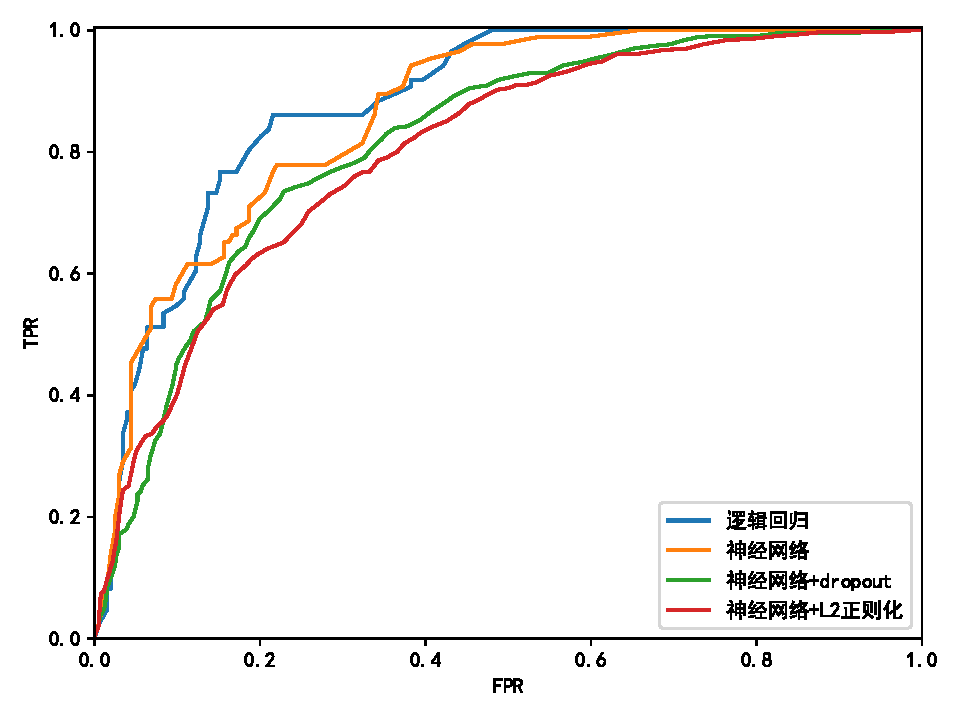
\includegraphics[width=\textwidth]{figure/f5.pdf}
	\caption{逻辑回归和神经网络的ROC曲线}
	\label{figure:ROC曲线}
\end{figure}
\begin{figure}[htbp]
	\centering
	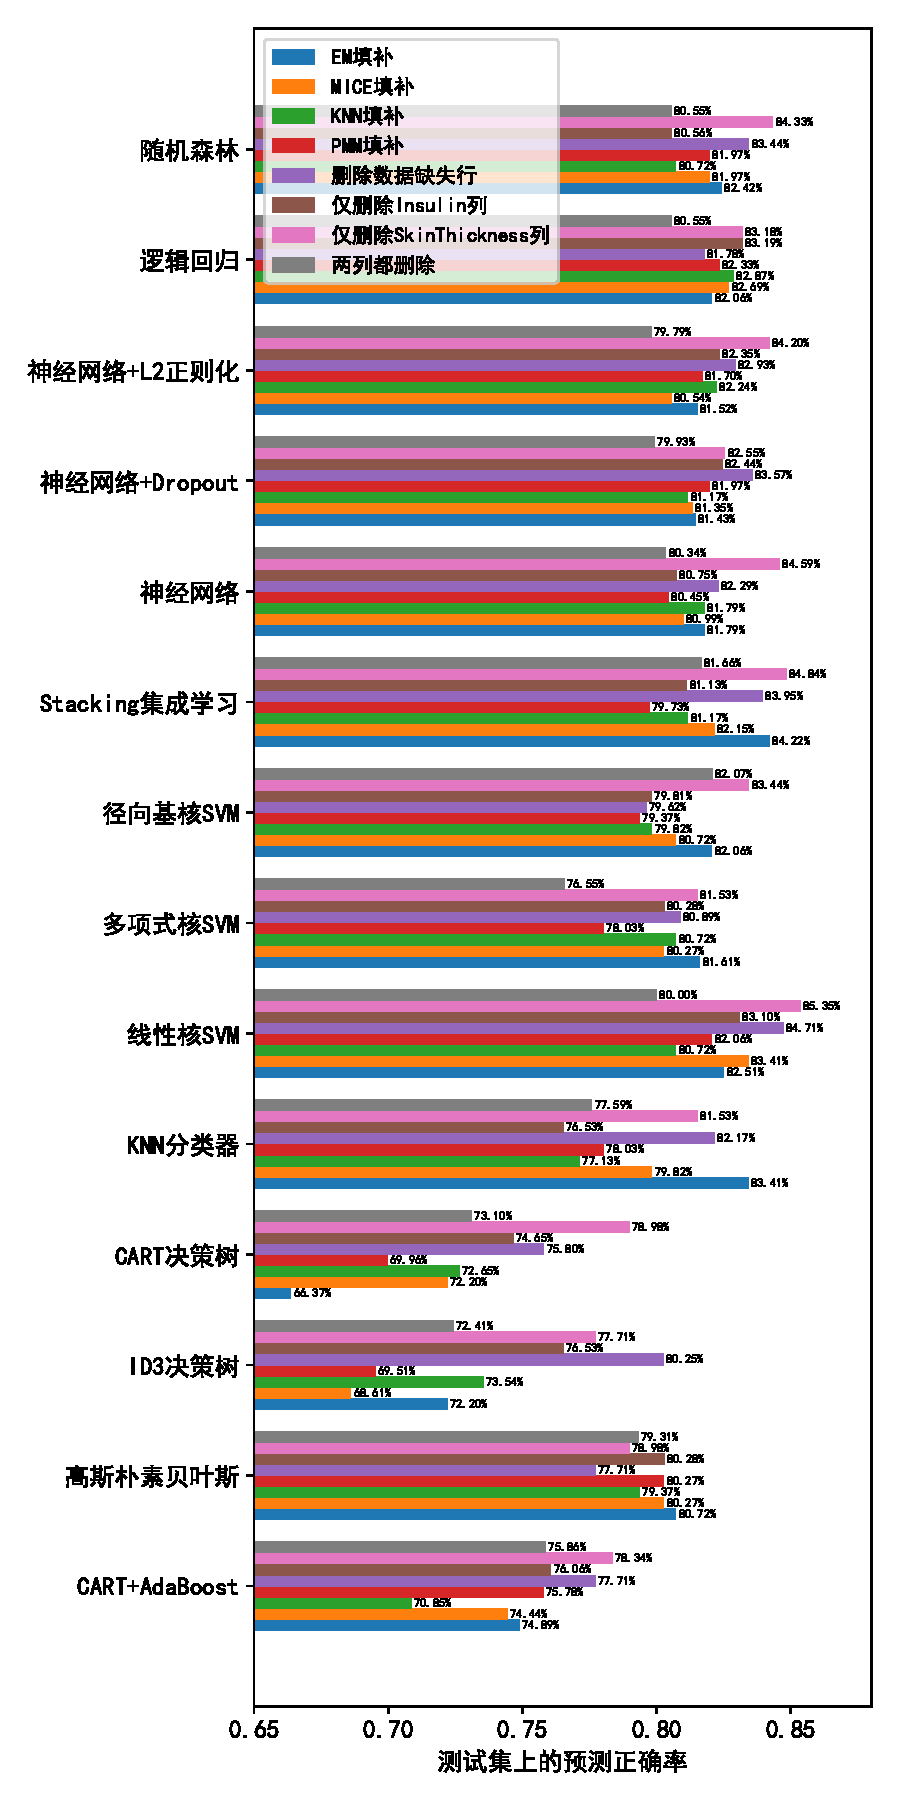
\includegraphics[width=0.8\textwidth]{figure/f1.pdf}
	\caption{各机器学习算法的准确率(以机器学习算法分组)}
	\label{figure:总体正确率}
\end{figure}
\begin{figure}[htbp]
	\centering
	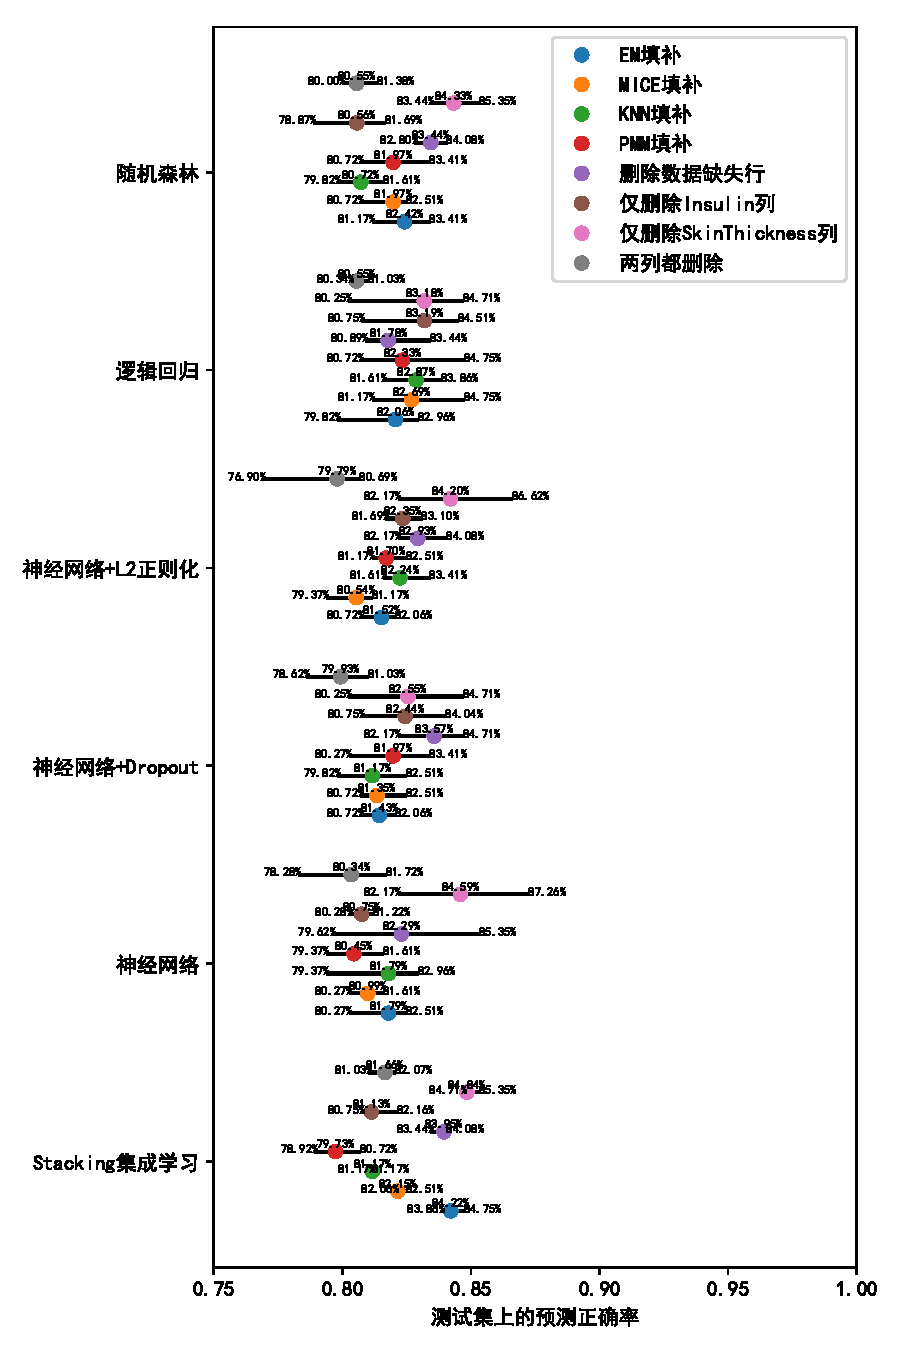
\includegraphics[width=\textwidth]{figure/f2.pdf}
	\caption{各机器学习算法的准确率均值和波动(以机器学习算法分组)}
	\label{figure:网络总体正确率}
\end{figure}
\begin{figure}[htbp]
	\centering
	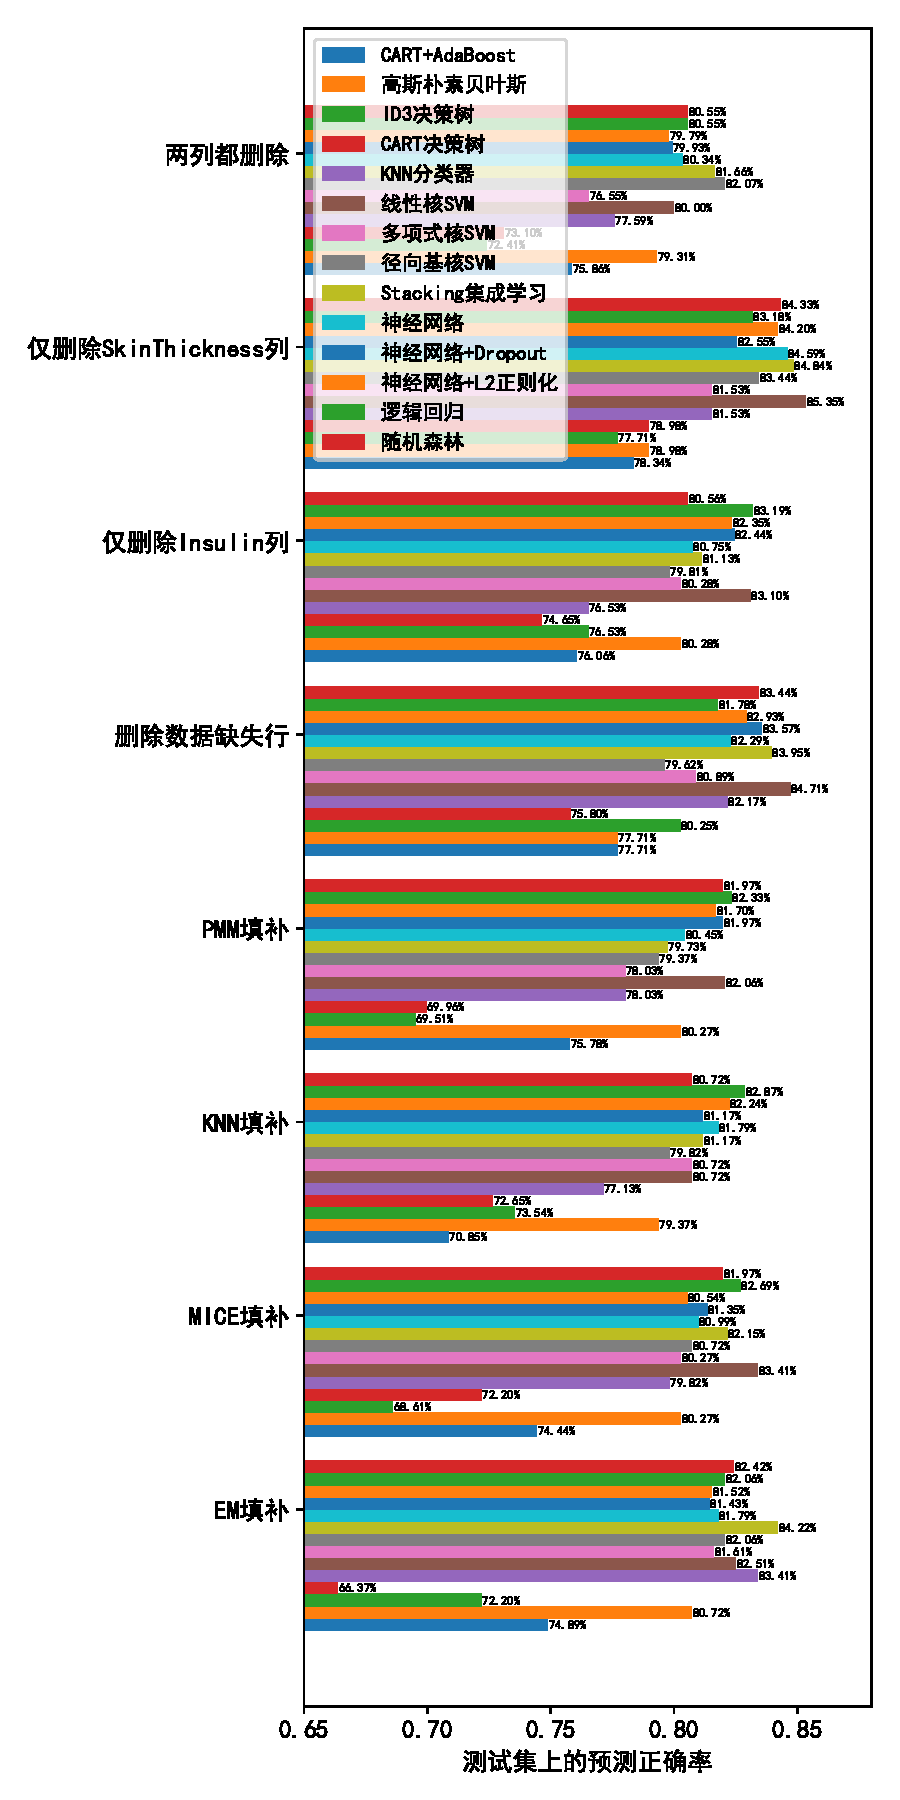
\includegraphics[width=0.8\textwidth]{figure/f3.pdf}
	\caption{各机器学习算法的准确率(以预处理方法分组)}
	\label{figure:数据集正确率}
\end{figure}
\begin{figure}[htbp]
	\centering
	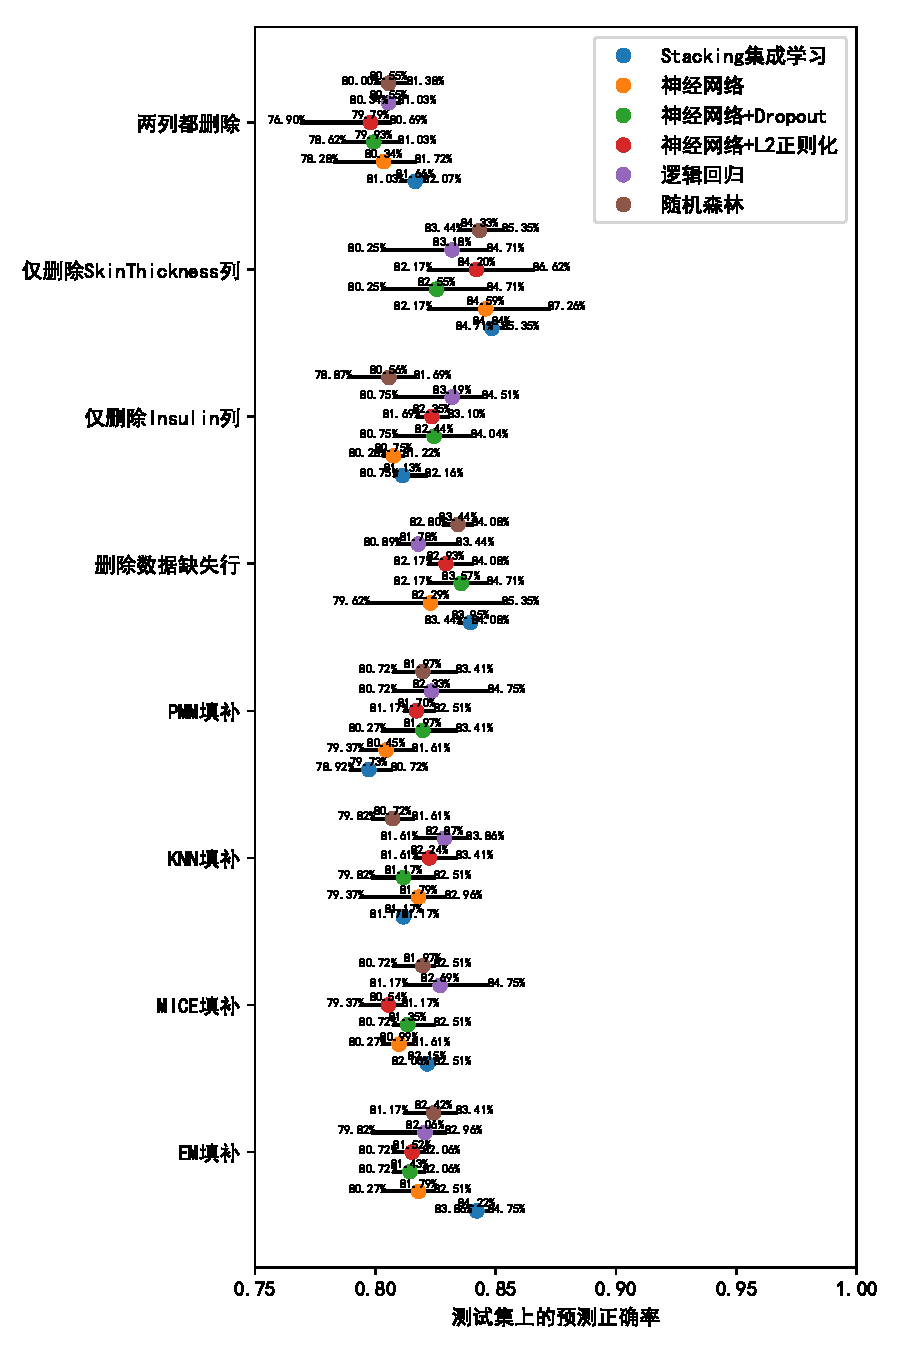
\includegraphics[width=\textwidth]{figure/f4.pdf}
	\caption{各机器学习算法的准确率均值和波动(以预处理方法分组)}
	\label{figure:网络数据集正确率}
\end{figure}

\newpage
\subsection{实验结果分析}
\begin{enumerate}
	\item 由表\ref{tab:混淆矩阵}可以看出:
	\begin{enumerate}[label=\alph*)]
		\item 错误估计的样本中假正例率和假负例率基本保持平衡,说明该算法对于正例和负例的判定都有比较好的结果;
		\item 正确估计的样本中主要都集中于真负例,说明该数据集的正负例非常不平衡;
		\item 上面两个结论表明,该算法在一个正负例不平衡的数据集中训练得到了一个假正例率和假负例率基本保持平衡的分类器,说明该算法具有很好的鲁棒性。
	\end{enumerate}
	\item 由图\ref{figure:ROC曲线}、图\ref{figure:总体正确率}和图\ref{figure:网络总体正确率}可以看出:
	      \begin{enumerate}[label=\alph*)]
		      \item 逻辑回归模型在该数据集上的准确性要略高于神经网络模型,且Dropout和L2正则化能使得神经网络模型的准确性和稳定性都有一定程度的提升,这说明本次实验中建立的神经网络模型在数据集上已经出现了过拟合现象,也印证了Dropout和L2正则化对神经网络模型过拟合的抑制作用;
		      \item 在三种使用不同核函数的SVM分类算法中,使用较为复杂的径向基核和多项式核构造SVM的分类正确率都不及最简单的线性核SVM,表明所使用的数据集中数据分布结构比较简单,复杂的核函数并不能对SVM分类准确率的提升有帮助;
		      \item 两种决策树算法在不同预处理数据集上的预测正确率相差很大,这表明决策树算法是一种不稳定的分类算法,在实际使用时需要一些后剪枝算法进行辅助\cite{dwyer2007decision};
			  \item 高斯朴素贝叶斯算法在不同的预处理数据集上都有大致相近的正确率,表明基于贝叶斯的分类算法具有较好的稳定性;
			  \item Stacking集成学习在多次重复实验中具有最高的稳定性,随机森林和AdaBoost集成学习算法在不同预处理数据集上的结果要比两种决策树算法都更接近,且随机森林算法的正确率要高于两种决策树算法,表明集成学习策略能提高机器学习算法的鲁棒性和准确性。
	      \end{enumerate}
	\item 由图\ref{figure:数据集正确率}和图\ref{figure:网络数据集正确率}可以看出:
	      \begin{enumerate}[label=\alph*)]
		      \item 经过EM填补的训练集训练出的机器学习算法在测试集上的准确率较为接近,且该训练集训练出的逻辑回归与神经网络算法在该测试集上的结果波动较小,表明EM填补相对于其他方法填补得到的训练集具有更好的分类特征,且不会与原数据集产生较大差异,对于有缺失数据的数据集使用EM算法能在一定程度上有提高训练出的机器学习算法的稳定性;
		      \item 删除“SkinThickness”列后的训练集训练出的逻辑回归与神经网络算法的测试集正确率较高但是波动很大,表明SkinThickness列并非是和糖尿病直接相关的特征,但是在一定程度上有助于糖尿病诊断;
		      \item 当删除训练集“Insulin”列或是“Insulin”和“SkinThickness”列都被删除时,逻辑回归与神经网络算法的测试集正确率都有所下降,这表明胰岛素确实时糖尿病诊断的重要特征。
	      \end{enumerate}
\end{enumerate}

\section{心得体会}
\begin{enumerate}
	\item 在实践中学习到了机器学习数据挖掘的流程和要点;
	\item 从实验结果中直观地感受到了各类机器学习算法的不同特点;
	\item 在机器学习算法的选择和使用方面积累了一定的经验;
	\item 将前两次作业中学到的理论知识付诸实践,对机器学习算法的主流理论有了更深入的理解;
	\item 经过课堂上的学习和这三次作业的梳理和实践,对机器学习和人工智能的主流理论及应用已经有了一个清晰的脉络和整体上的把握,对于在机器学习、人工智能和数据挖掘领域后续更加深入的学习已经形成了一个明确的方向。
\end{enumerate}

\bibliography{ref}
\end{document}